\chapter{Sistema Embebido}
\cleanchapterquote{No me dan miedo los ordenadores. Temo la falta de ellos}{Isaac Asimov}{(Escritor americano)}

En este capitulo se abordan los procedimientos de diseño del sistema embebido desde la parte mecánica hasta la
obtención del controlador.

\section{Arquitectura}
La arquitectura general del sistema embebido está dividido en 3 diferentes sub-áreas que en su conjunto ayudan al
seguimiento de un objetivo mediante visión artificial.
\begin{center}
	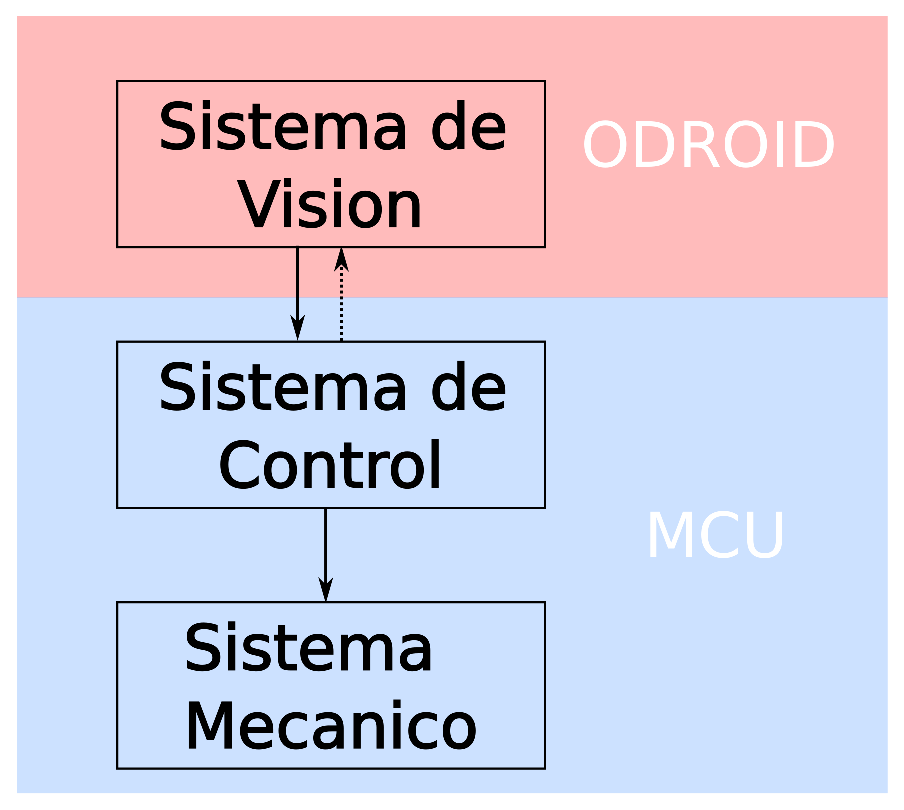
\includegraphics[width=0.45\textwidth]{Contenido/Cuerpo/Capitulo5/Fig12.eps}
	\captionof{figure}{Modulos del sistema}\label{Fig1}
\end{center}
Tal y como se ilustra en la figura 5.1, dichas áreas se relacionan entre si, compartiendo datos para tener un
sistema integrado y robusto.
\begin{itemize}
	\item Visión: Identifica el centroide del objetivo, el desarrollo del algoritmo se abordó en el capítulo 4. Interacciona con el sistema de control enviando la retroalimentación
	      y recibe de este ultimo datos del error.
	\item Control: Un micro-controlador es el encargado de interactuar con los datos de la cámara y retroalimentarlos con la
	      salida deseada, para después controlar con un PI.
	\item Mecánico: Son los actuadores del sistema que hacen que la cámara tenga dos grados de libertad de movimiento, que
	      son las rotaciones en Pitch y Yaw, el modelo se abordó en el Capitulo 3.
\end{itemize}
La comunicación de datos se da por varios buses de datos, entre todos los componentes del sistema, la figura 5.2 ilustra
la interacción entre ellos y se presenta la arquitectura propuesta
\begin{center}
	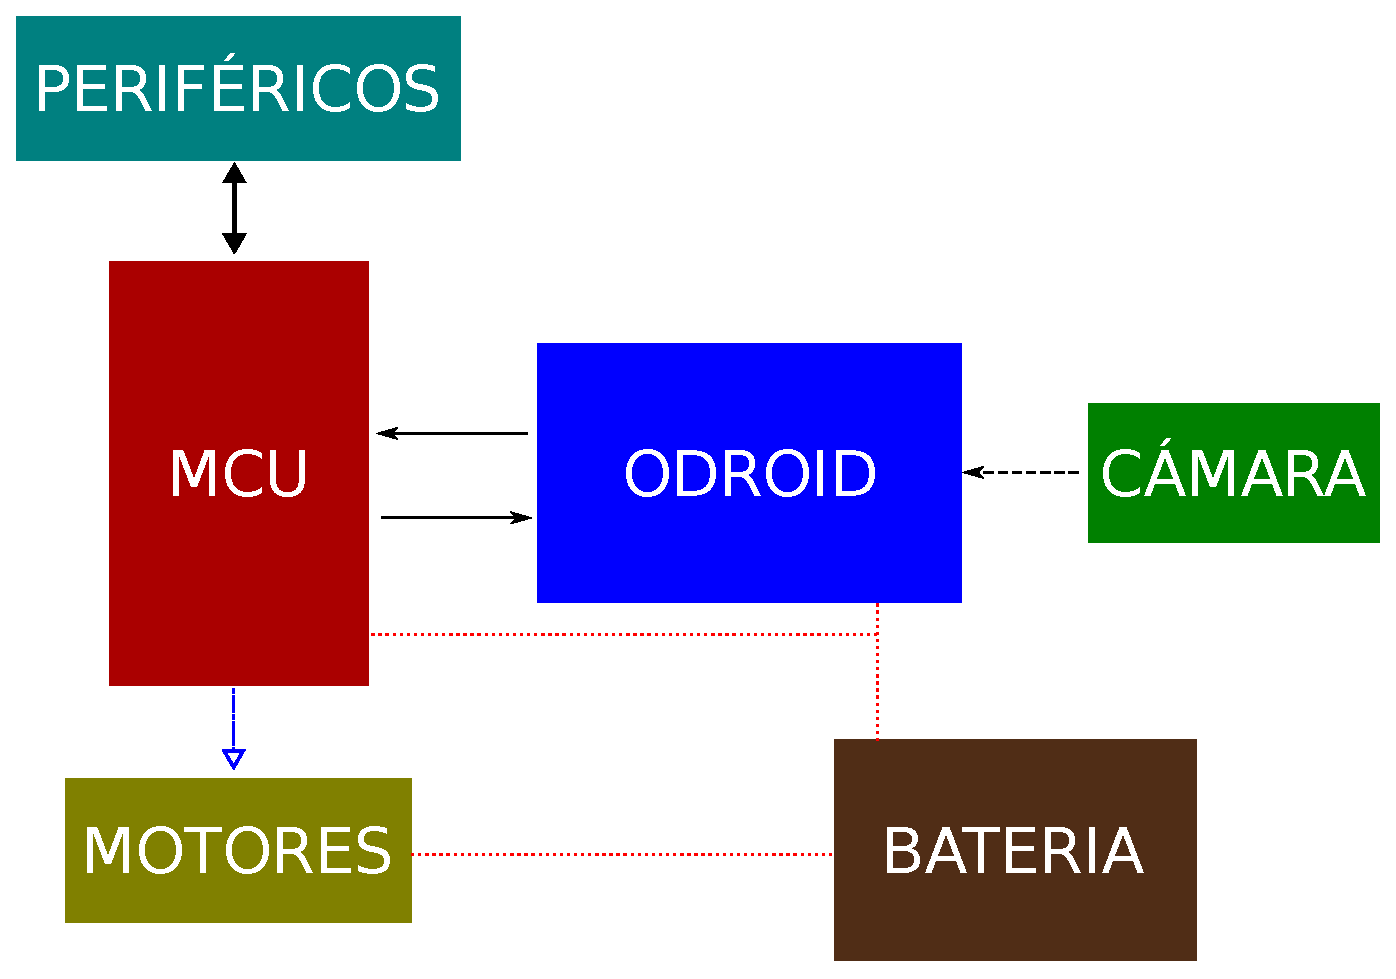
\includegraphics[width=0.5\textwidth]{Contenido/Cuerpo/Capitulo5/Fig13.eps}
	\captionof{figure}{Arquitectura del sistema}\label{Fig1}
\end{center}
El microcontrolador es de 32 bits arquitectura RISC, las especificaciones detalladas de los motores y de la tarjeta de desarrollo
ODROID puede ser consultada en el Apéndice B.\\
El Bus señalado con líneas punteadas en rojo representan la conexión de voltaje con los demás componentes, mientras que la línea punteada en negro entre la cámara y la odroid
simboliza la conexión USB para la transferencia de datos, la comunicación entre ODROID y el MCU se da mediante el módulo RS-323 integrado en el microcontrolador que a su vez
se comunica con los periféricos deseados utilizando sus salidas digitales.\\
Este tipo de Arquitectura permite que la ODROID pueda comunicarse paralelamente con el MCU por medio del protocolo serial, que va
a 57000 baudios, además de que permite que el microcontrolador tenga la posibilidad de publicar en ROS.

% ---------------------------------------------------------------------------------------------------------
% *********************************************************************************************************
% *********************************************************************************************************
% ---------------------------------------------------------------------------------------------------------


\section{Mecanismo móvil}
El diseño del sistema fue hecho mediante el uso de software libre llamado OpenSCAD, en el cual se trazó el prototipo del
sistema utilizando dos motores tipo servo, es decir, que tienen su propio controlador de velocidad integrado vía PWM.
\begin{center}
	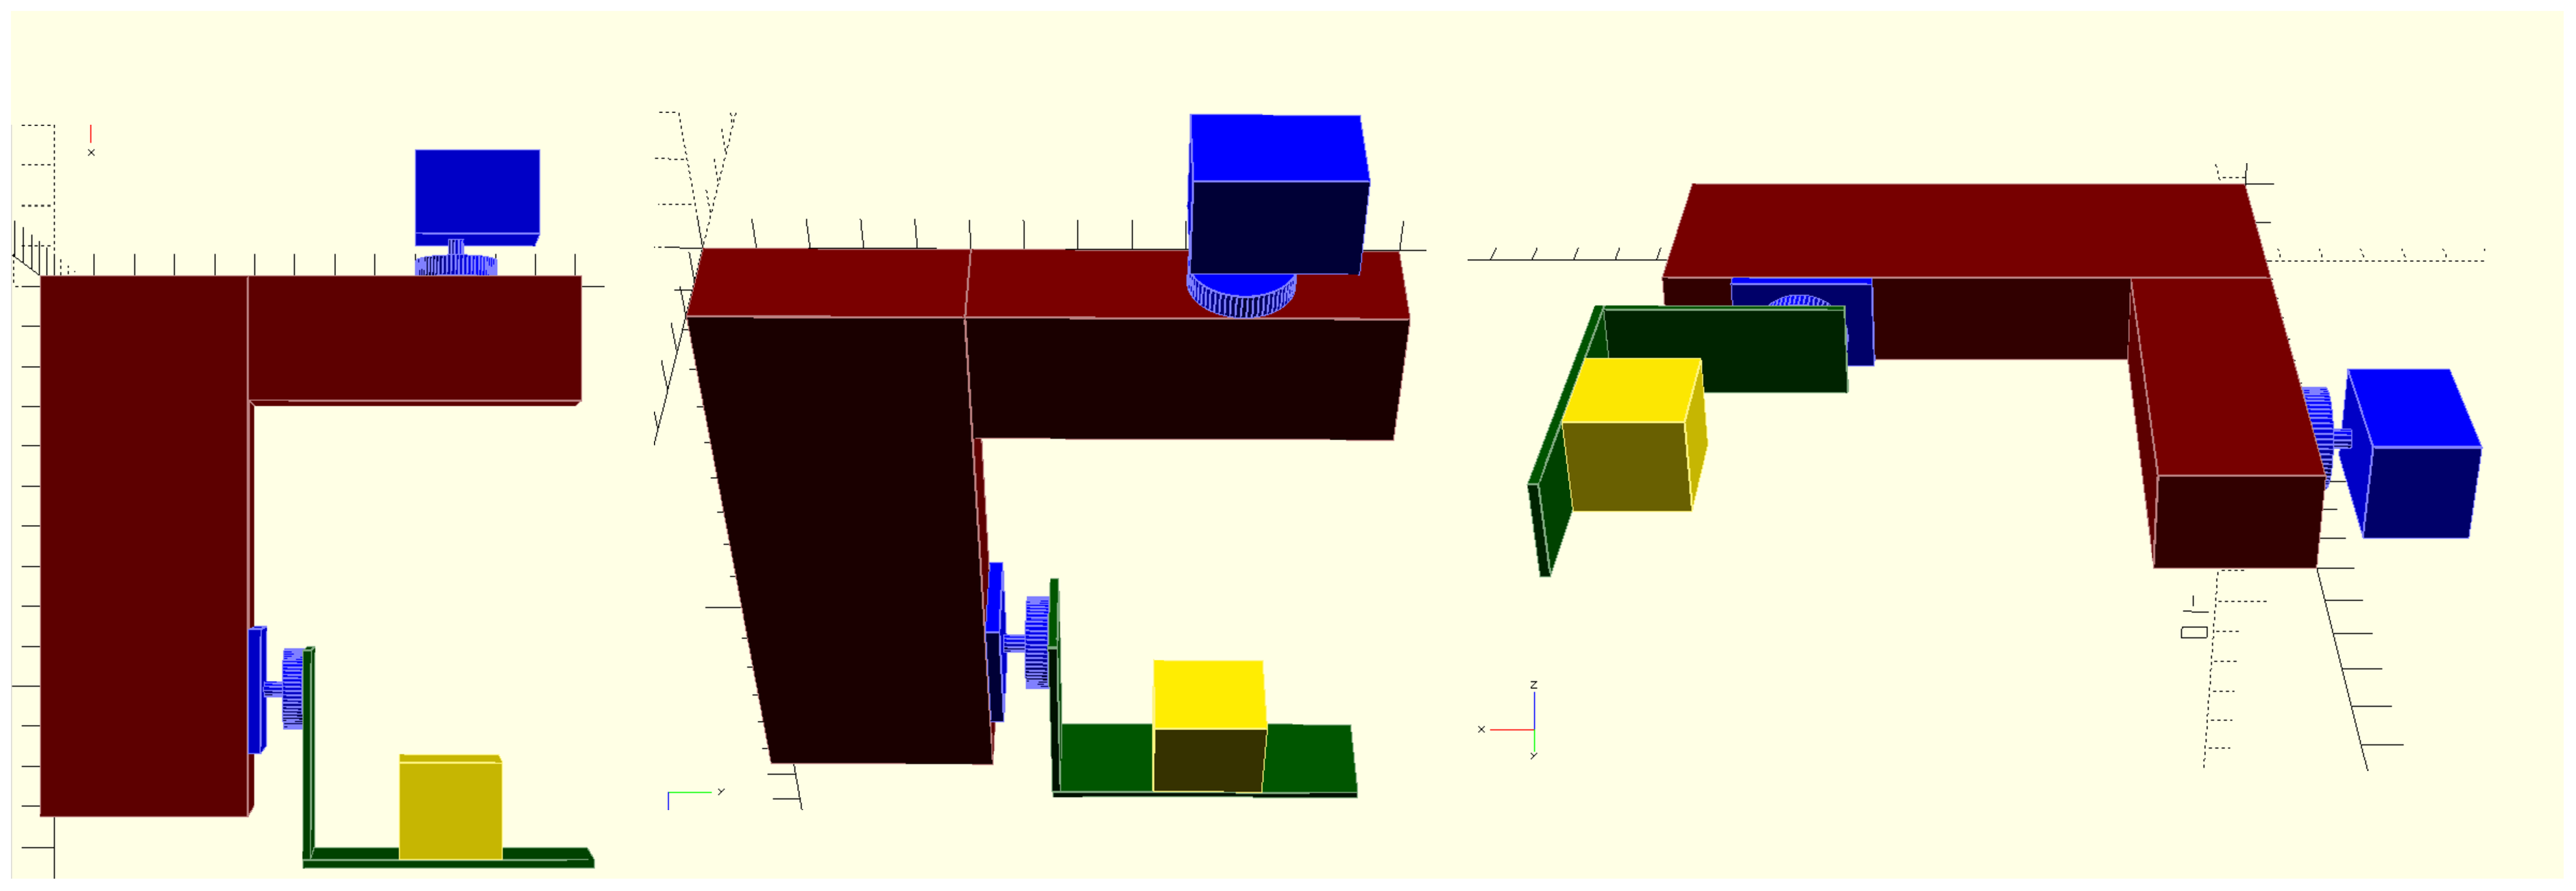
\includegraphics[width=1.0\textwidth]{Contenido/Cuerpo/Capitulo5/Fig14.eps}
	\captionof{figure}{Diseño CAD del prototipo}\label{Fig1}
\end{center}
En la figura 5.3 los motores están representados en color azul, mientras que la cámara esta de amarillo, como se puede apreciar
la cámara recae sobre un soporte de color verde, dicha cámara está sujeta por un par de ligas que ayudan a que esta no se
caiga cuando hay rotación en pitch\\
A continuación en la figura 5.4 se presentan algunas medidas del diseño, las unidades están en mm.
\begin{center}
	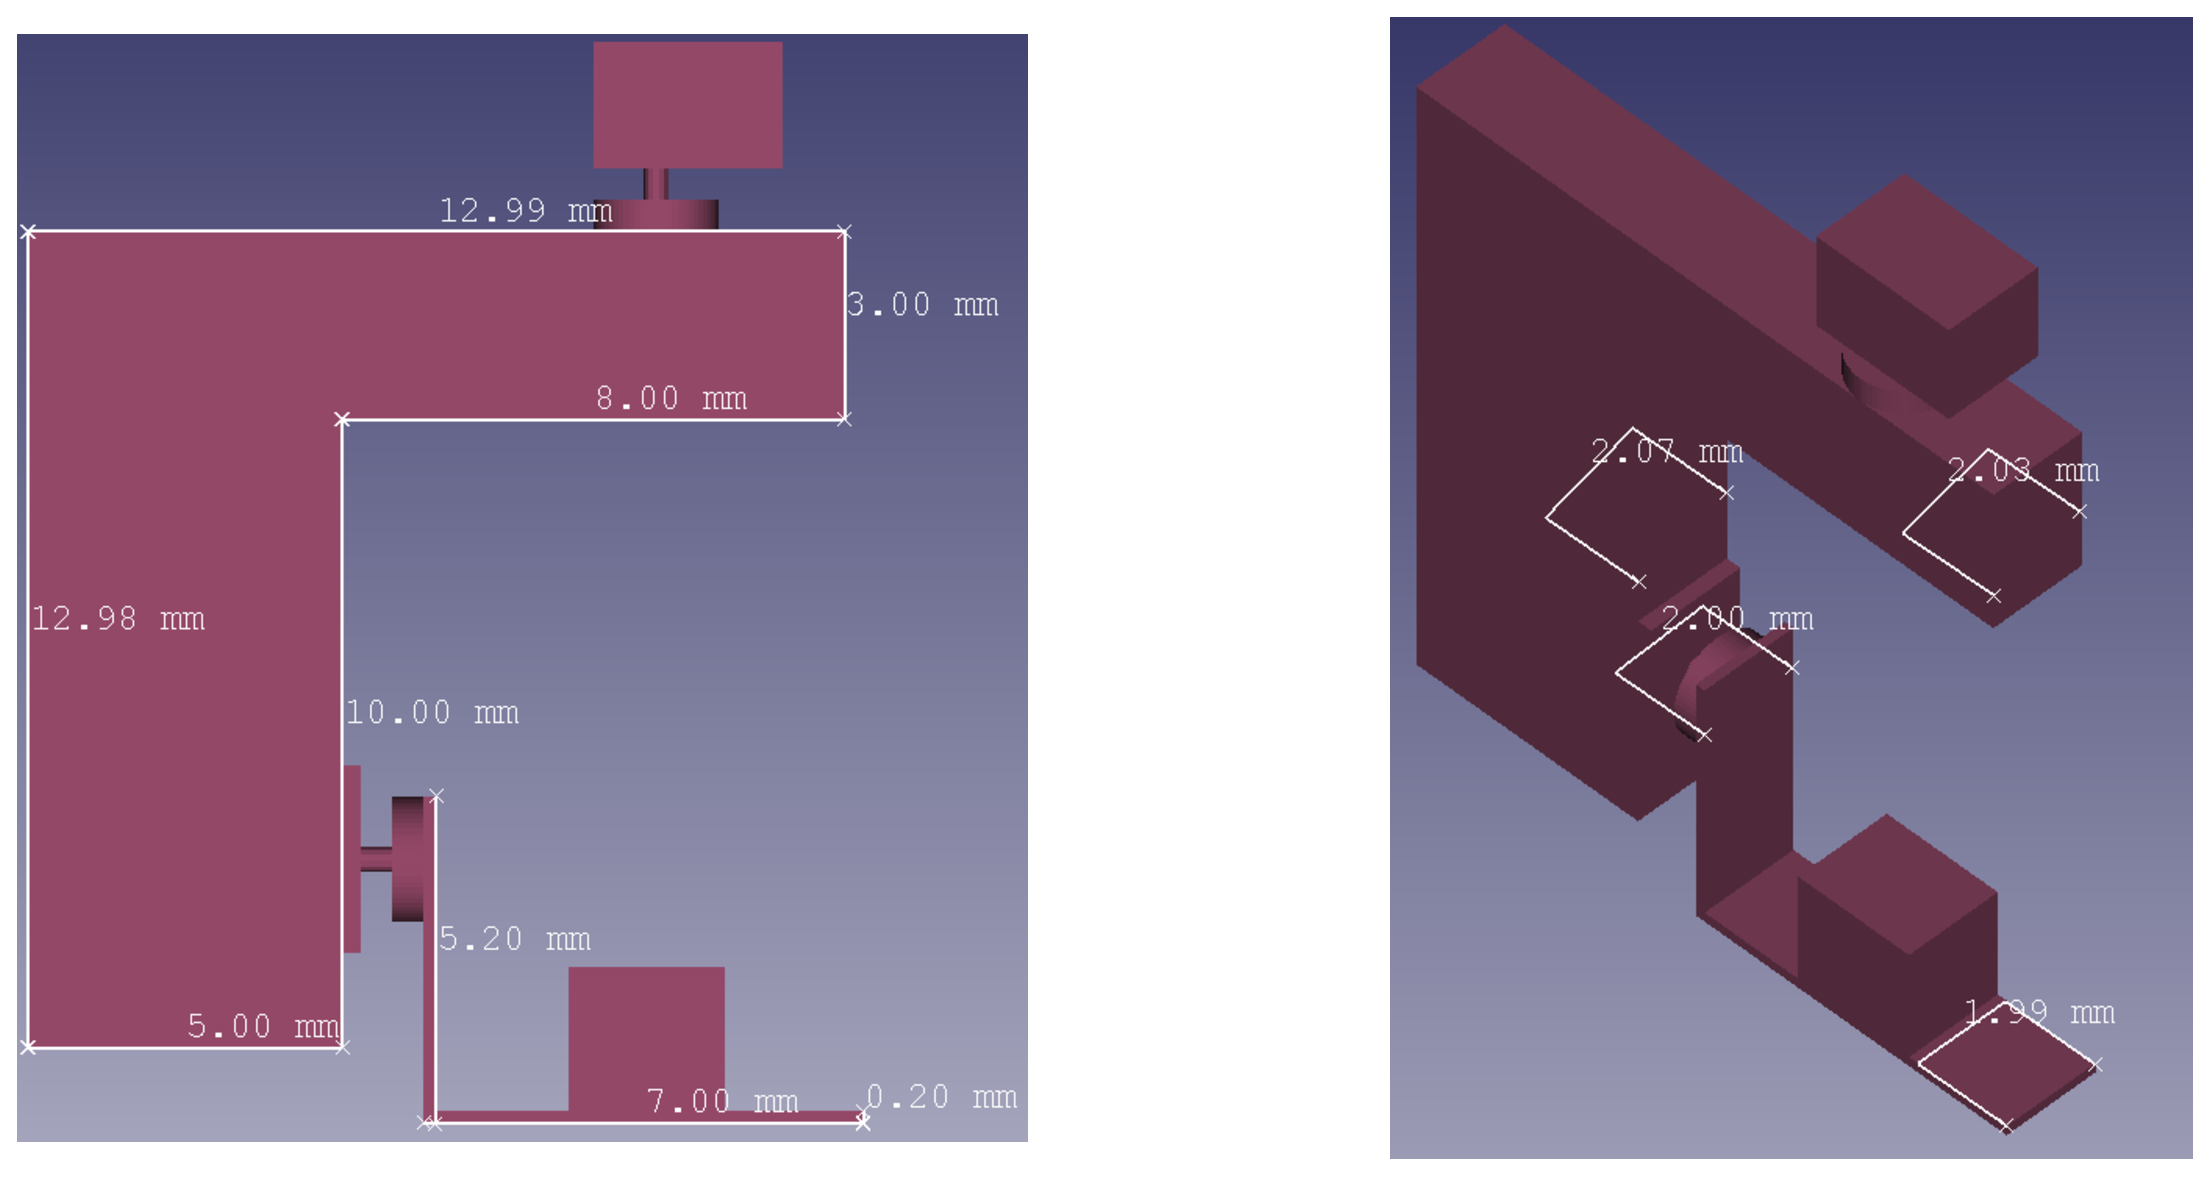
\includegraphics[width=0.8\textwidth]{Contenido/Cuerpo/Capitulo5/Fig16.eps}
	\captionof{figure}{Dimensiones del CAD}\label{Fig1}
\end{center}
Como se vio previamente en los capítulos 2 y 3 este sistema tendrá dos ejes de libertad, que en términos técnicos, a estos
movimientos también se les conoce como "\ Till \" y "\ Pan \" que es no es mas que otra manera de decirle a la rotación
sobre el eje Y y Z.\\
Es entonces que esos movimientos pueden ser visualizados como se presenta en la figura 5.5.
\begin{center}
	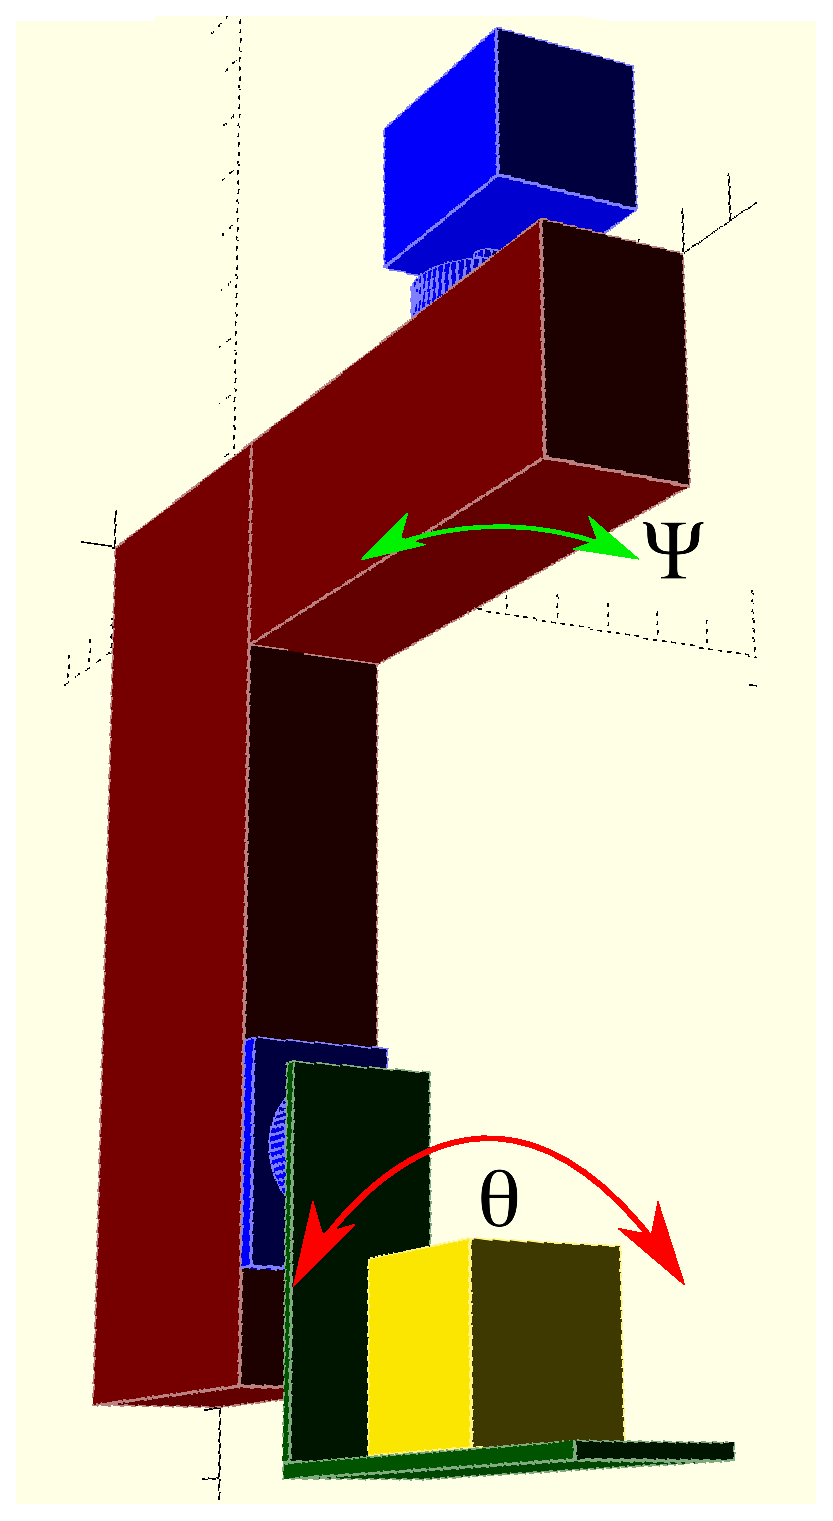
\includegraphics[width=0.35\textwidth]{Contenido/Cuerpo/Capitulo5/Fig15.eps}
	\captionof{figure}{Grados de libertad del sistema}\label{Fig1}
\end{center}
Donde
\begin{itemize}
	\item $\theta$ representa el movimiento de "\ Till "
	\item $\psi$ representa el movimiento de "\ Pan  "
\end{itemize}

% ---------------------------------------------------------------------------------------------------------
% *********************************************************************************************************
% *********************************************************************************************************
% ---------------------------------------------------------------------------------------------------------
\section{Prototipo físico}
Para la realización del prototipo se utilizó un material ligero para que no agregue mucho peso adicional al sistema.
\begin{center}
	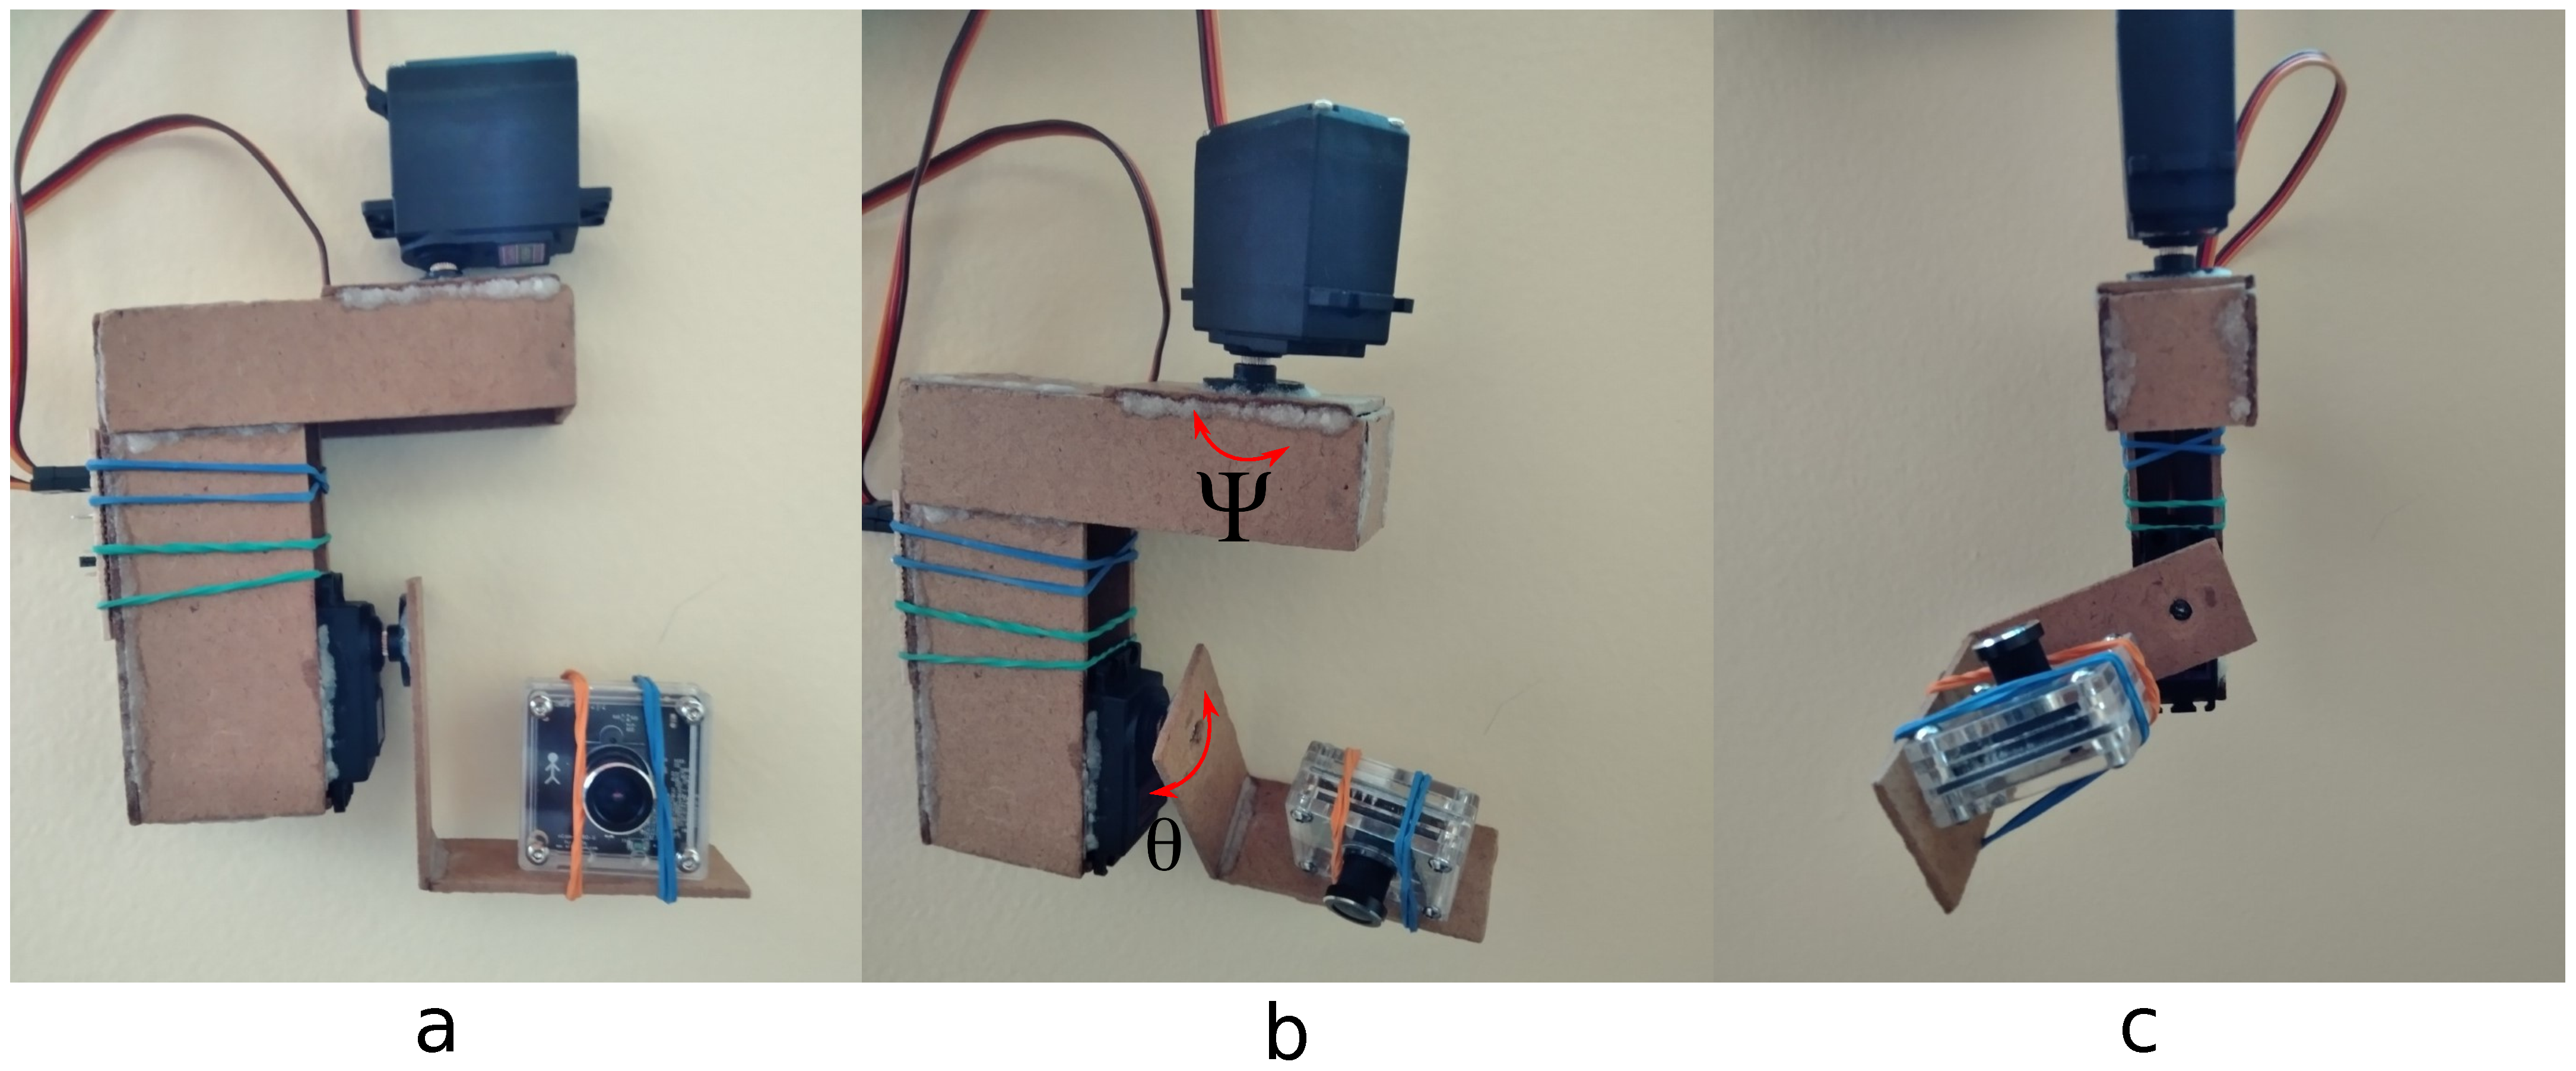
\includegraphics[width=0.8\textwidth]{Contenido/Cuerpo/Capitulo5/Fig17.eps}
	\captionof{figure}{Prototipo del sistema hecho con madera}\label{Fig1}
\end{center}
Como se puede observar en la figura 5.6 la cámara esta sujeta a la base por medio de ligas que le dan mejor soporte y ayudan a que
esta no se caiga al momento de seguir a los objetivos.
\begin{itemize}
	\item Peso del sistema sin motores ni cámara : 70 g
	\item Peso con motores y cámara : 215 g
\end{itemize}
En b) y c) de la figura 5.6 se ilustra el movimiento que puede realizar el sistema, y que será controlado
por la cámara y actuado por los motores.\\
Adicionalmente se diseñó un pequeño circuito que sirve como terminal para las conexiones de alimentación y señales,
dicho circuito se encuentra en la parte lateral del sistema sujetado por ligas y pegamento.\\
La conexiones eléctricas se ilustra en la figura 5.7. Es una esquemático que muestra la conexión entre los componentes principales: la cámara(OCAM), monoprocesador(ODROID),
el microcontrolador (ATMEGA) y los motores (Servomotores)
\begin{center}
	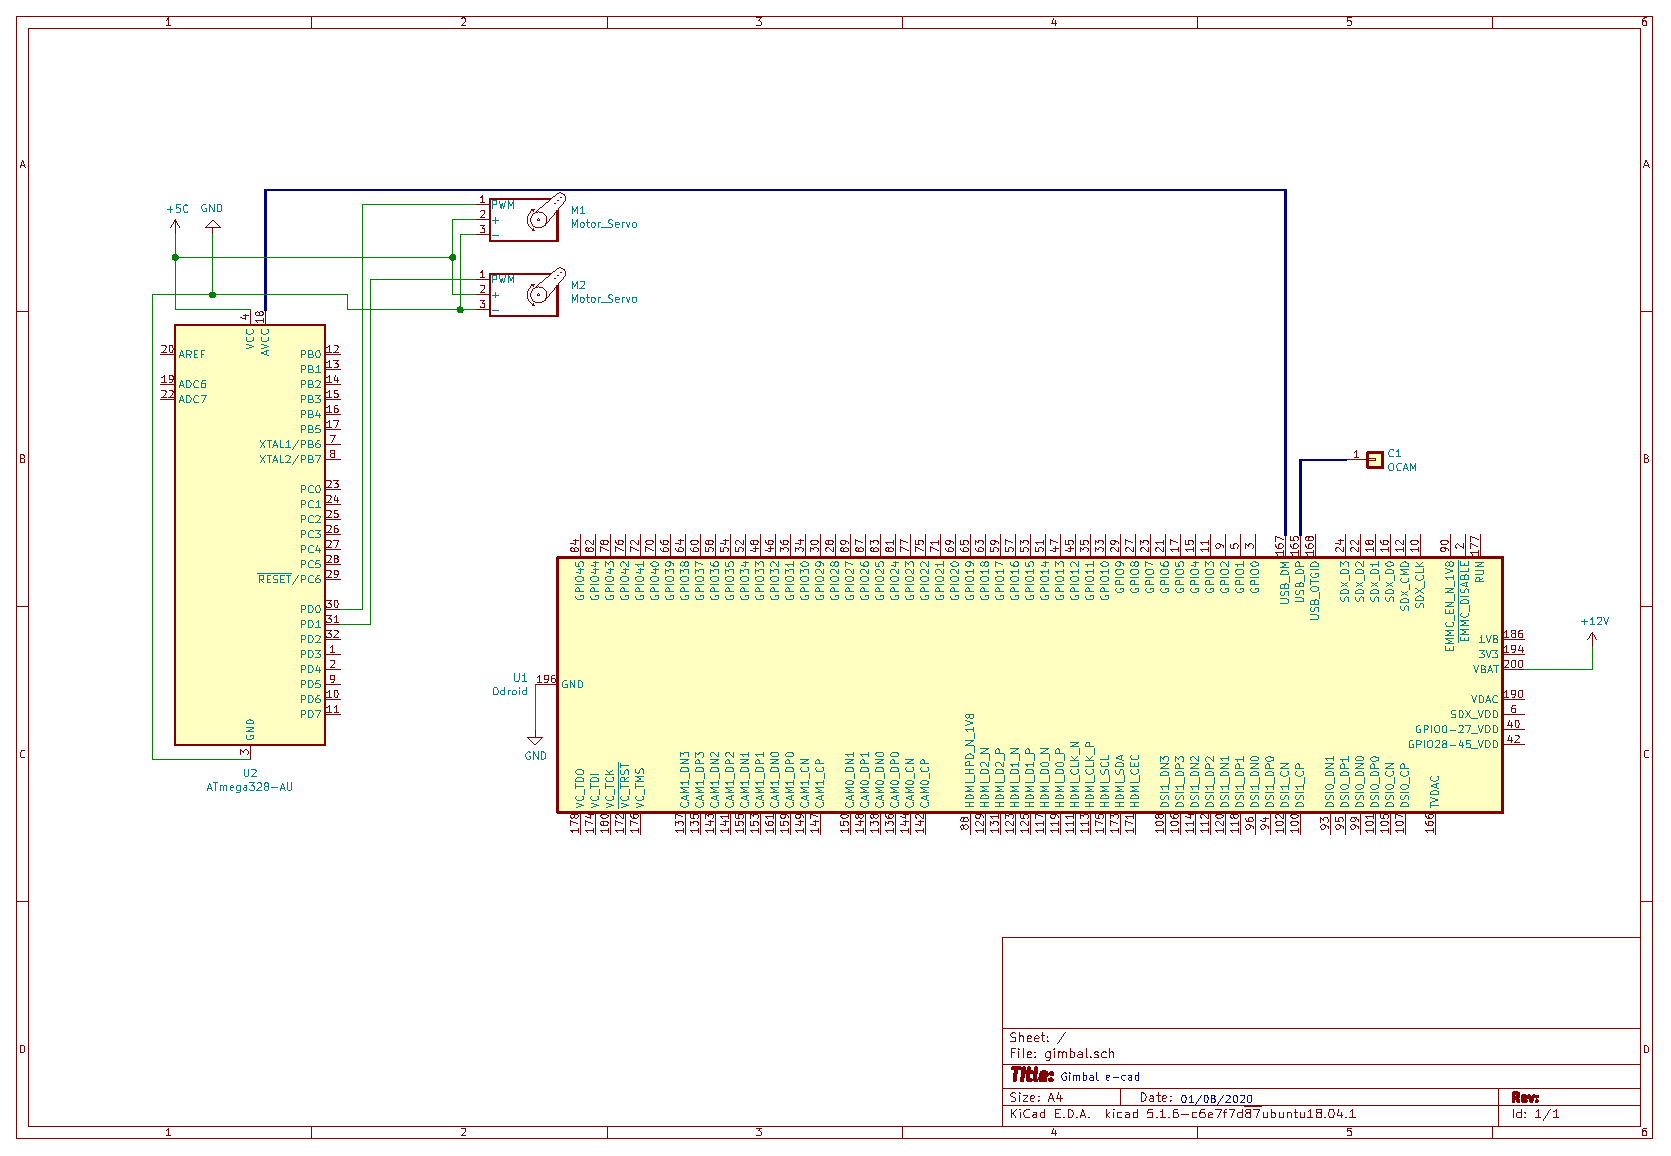
\includegraphics[width=1.0\textwidth]{Contenido/Cuerpo/Capitulo5/Fig21.eps}
	\captionof{figure}{Circuito eléctrico}\label{Fig1}
\end{center}


% ---------------------------------------------------------------------------------------------------------
% *********************************************************************************************************
% *********************************************************************************************************
% ---------------------------------------------------------------------------------------------------------


\section{ROS-Microcontrolador}
La parte mecánica encargada de hacer mover la cámara alrededor de dos ejes son los motores de corriente directa, que están conectados
a un microcontrolador que es el encargado de ejecutar el controlador.\\
El control tiene como entrada las coordenadas obtenidas por el algoritmo descrito en el capitulo 4. Y con base en ese pixel, podemos
calcular el error teniendo en cuenta que la referencia es el centro de la cámara.\\
Una vez dicho lo anterior queda una pregunta clara, ¿Como comunicar el microcontrolador encargado de los motores, con la cámara que
esta siendo ejecutada en ROS?
\begin{center}
	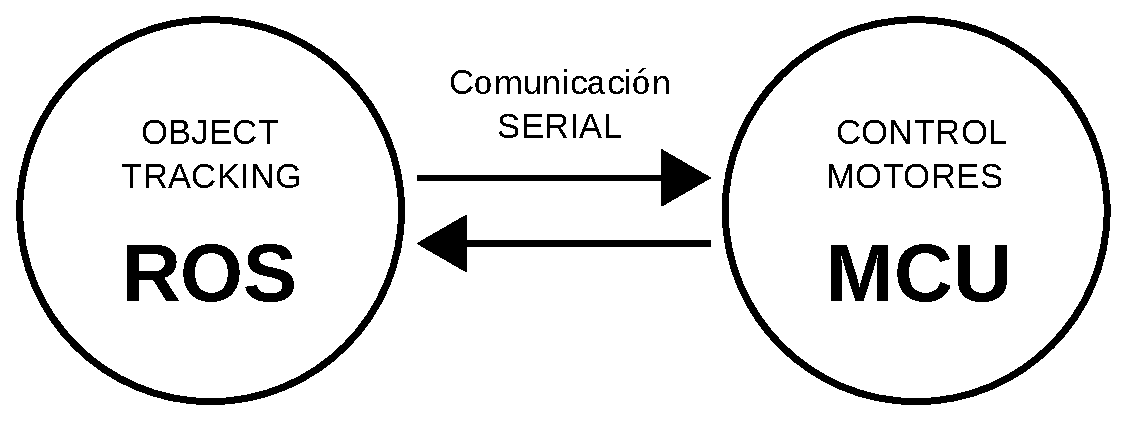
\includegraphics[width=0.45\textwidth]{Contenido/Cuerpo/Capitulo5/Fig1.eps}
	\captionof{figure}{Protocolo de comunicación}\label{Fig2}
\end{center}
Como se ilustra en la imagen anterior el protocolo de comunicación que se utilizó es el serial, debido a su practicad y que ya
cuenta con librerías de ROS para el microcontrolador, que para la primera etapa de esta investigación se utiliza el Atmega328p.\\
La comunicación esta basado en ser asíncrona, y se detalla mejor en el siguiente diagrama:
\begin{center}
	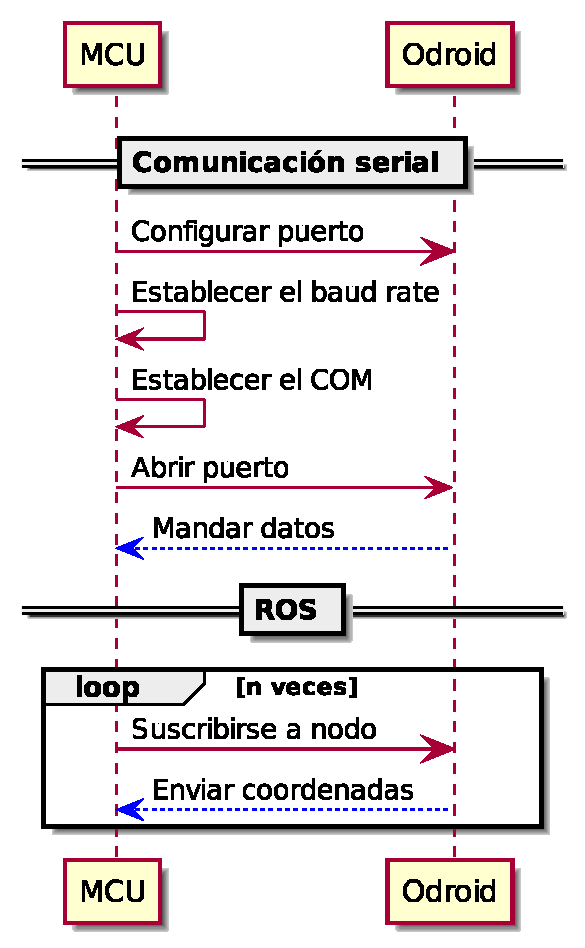
\includegraphics[width=0.35\textwidth]{Contenido/Cuerpo/Capitulo5/Fig2.eps}
	\captionof{figure}{Diagrama de secuencia}\label{Fig3}
\end{center}
La velocidad de la comunicación es de 570000 baudios y se conecta a través de un cable usb. El microcontrolador tiene además
la función de publicar el error con la finalidad de graficar dicho error y obtener conclusiones. Que visto desde el plano
de ROS tenemos los siguientes Topics y Nodes:
\begin{center}
	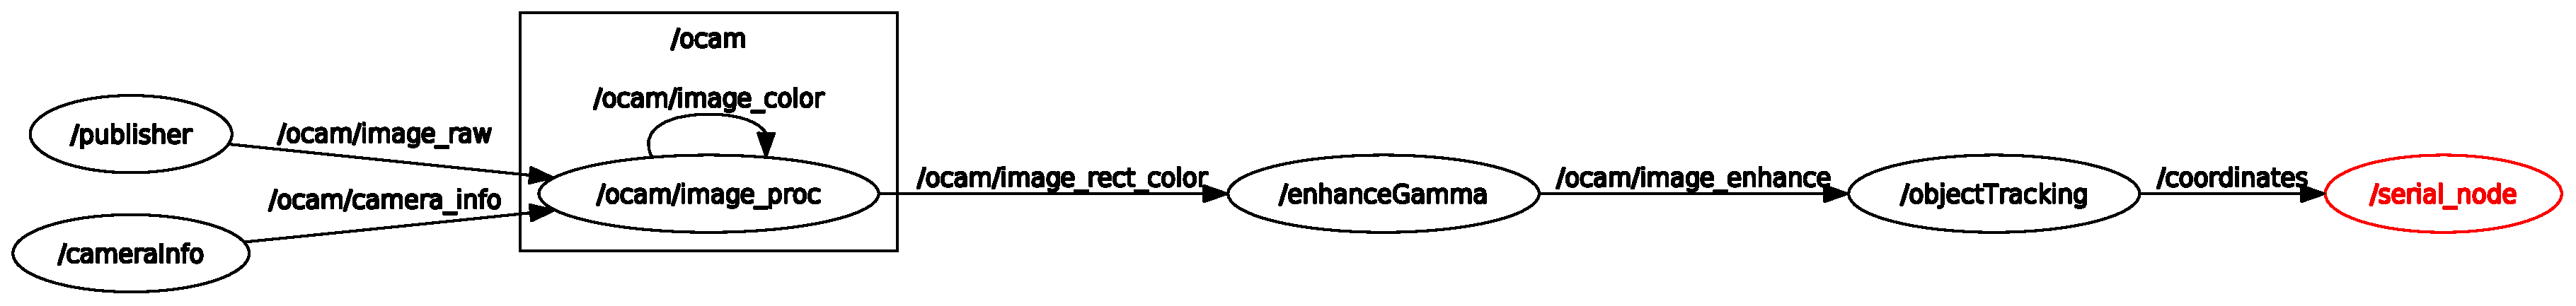
\includegraphics[width=0.9\textwidth]{Contenido/Cuerpo/Capitulo5/Fig3.eps}
	\captionof{figure}{Nodos y Topicos activos}\label{Fig4}
\end{center}


% ---------------------------------------------------------------------------------------------------------
% *********************************************************************************************************
% *********************************************************************************************************
% ---------------------------------------------------------------------------------------------------------


\section{Control}
La idea principal del sistema de control es la de encontrar una función de entrada $u(t)$ tal que la función de salida $x(t)$ siga a la
salida deseada $x^{des}(t)$. Para lograr esto vamos a utilizar la siguiente aproximación
\begin{equation}
	e(t) = x^{des}(t) - x(t)
\end{equation}
Donde $e(t)$ representa el error. Por lo que la estrategia es encontrar un $u(t)$ tal que
\begin{equation}
	K_i\int e + k_pe = 0
\end{equation}
Donde $k_i$ y $k_p$ $> 0$\\
Y tal y como se abordo en el capitulo 2 esto nos lleva al control Proporcional-Integral
\begin{equation}
	u(t) = k_i\int{e}(t) + k_pe(t)
\end{equation}

\subsection{Control servomotor}
Como vimos en el capítulo 3, la función de transferencia de un motor de corriente continua es de segundo orden, e involucra algunas constantes que dependen del toque máximo y
de la velocidad sin carga.
\begin{equation}
	\frac{\theta_m (s)}{E_a(s)} = \frac{K_t / (R_aJ_m)}{s \left[ s + \frac{1}{J_m} \left( D_m + \frac{K_tK_b}{R_a} \right) \right]}
\end{equation}
El motor que se utilizó para hacer el mecanismo móvil es el MG996R, es un motor de tipo servo 360 grados, esto quiere decir que da todo el giro, a diferencia de los servomotores
convencionales. Las especificaciones técnicas son las siguientes:
\begin{itemize}
	\item Peso = 55g
	\item Torque stall = 11kg/cm a 6v
	\item Velocidad sin carga = 0.14s/ 60° a 6v
	\item Voltaje de operación = 4.8v a 7.2v
	\item Temperatura de operación = 0°C - 55°C
	\item PWM = 20ms (50Hz) de operación
\end{itemize}
La siguiente gráfica muestra la relación que hay entre el torque y la velocidad, que como se puede observar es lineal. Esta grafica se obtuvo con los datos sugeridos del
provedor.
\begin{center}
	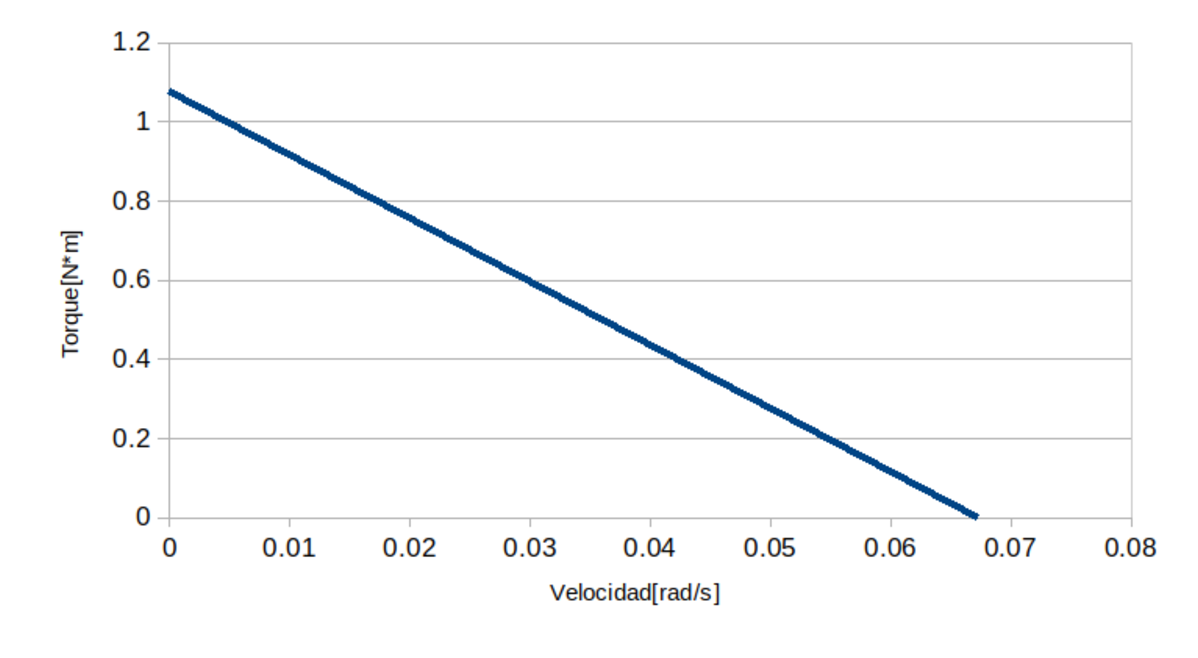
\includegraphics[width=0.8\textwidth]{Contenido/Cuerpo/Capitulo5/Fig19.eps}
	\captionof{figure}{Gráfica torque-velocidad}\label{Fig4}
\end{center}
Ahora encontraremos las constantes eléctricas, $K_t / R_a$ y $K_b$. De la curva de par-velocidad de la figura anterior
\begin{itemize}
	\item $T_{stall}$ = 1.078
	\item $\omega_{sincarga}$ = 0.0673
	\item $e_a$ = 6v
\end{itemize}
Las constantes electricas son
\begin{equation}
	\frac{K_t}{R_a} = \frac{T_{stall}}{e_a} = \frac{1.078}{6} = 0.17966
\end{equation}
y
\begin{equation}
	K_b = \frac{e_a}{\omega_{sin carga}} = \frac{6}{0.0673} = 89
\end{equation}
La carga en cada motor es diferente, vamos a calcularla con al siguiente ecuacion del momento de inercia
\begin{equation}
	I = mr^2
\end{equation}
\begin{center}
	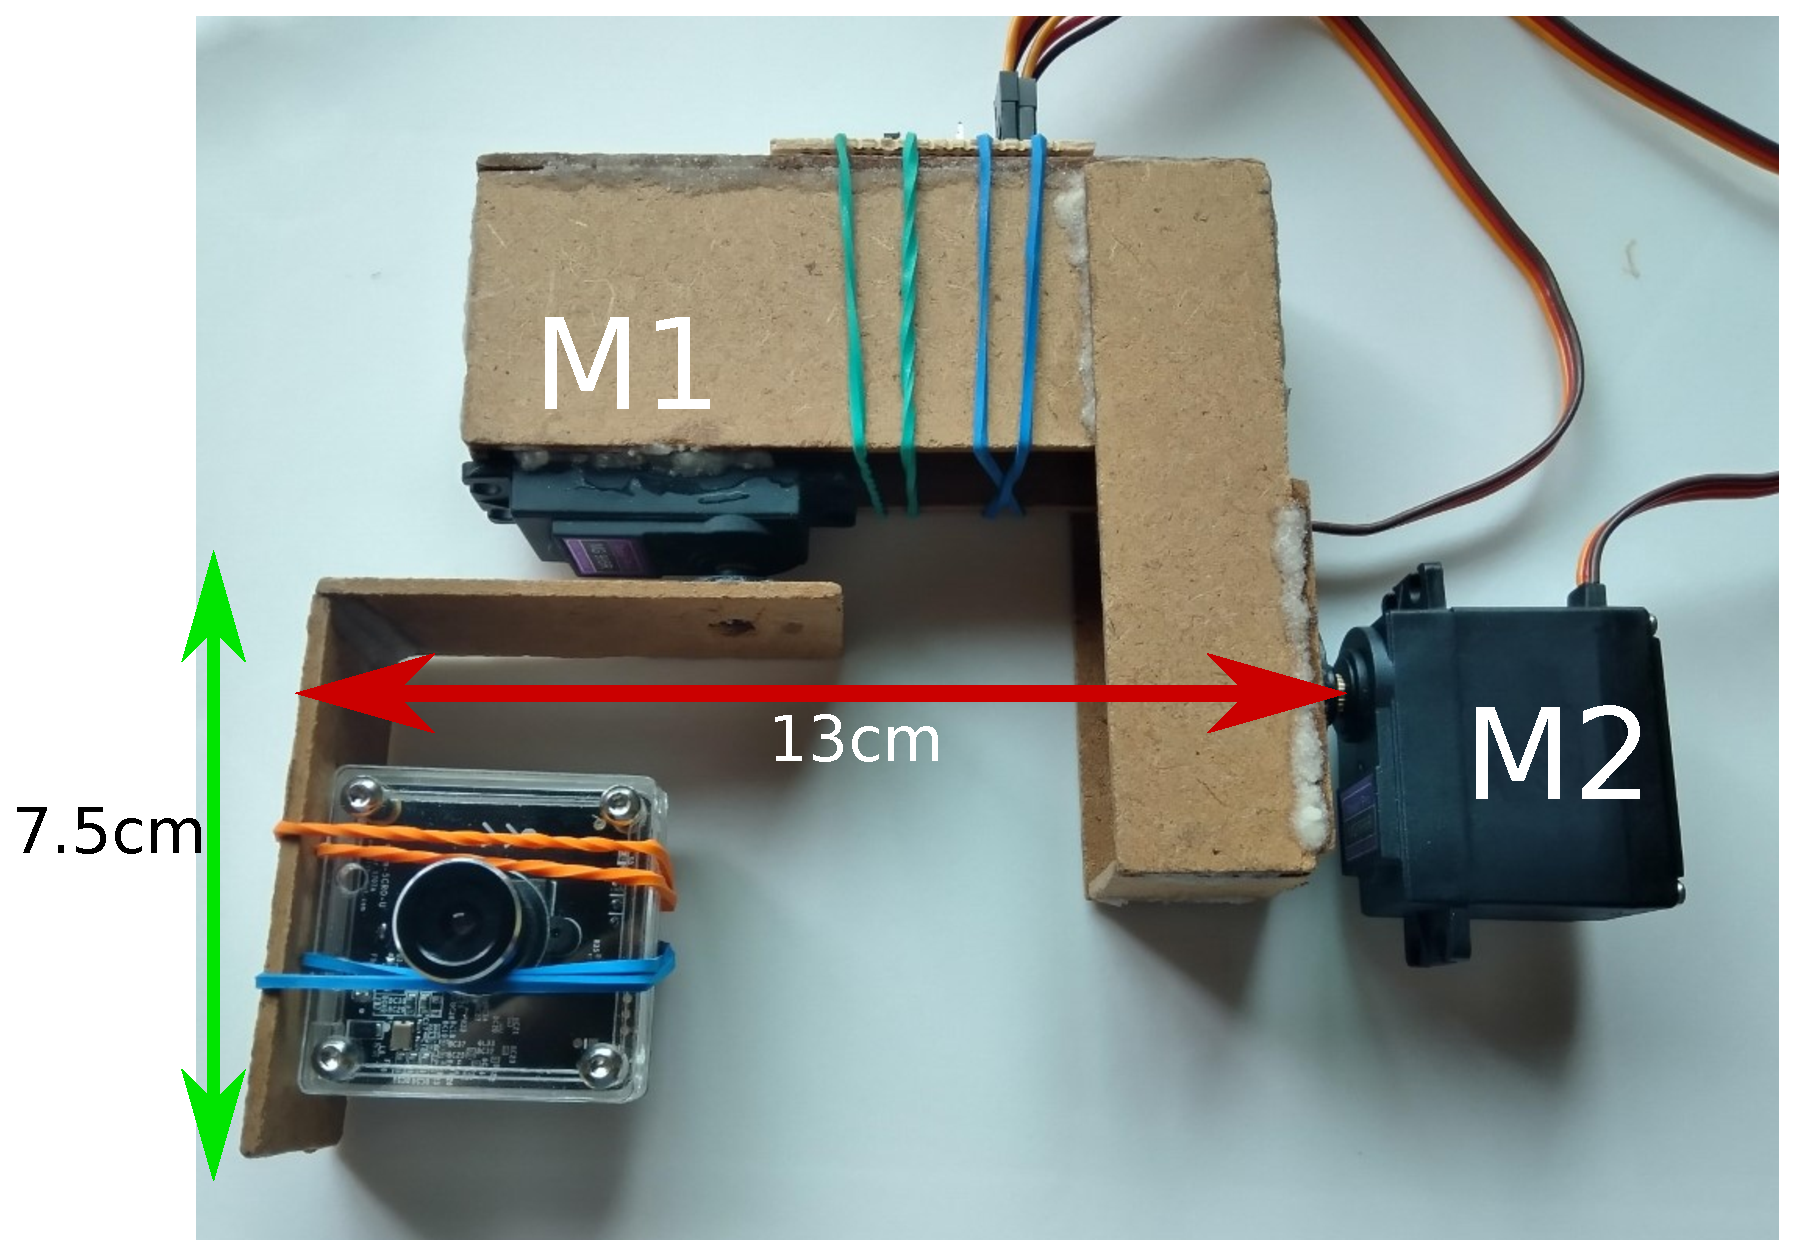
\includegraphics[width=0.6\textwidth]{Contenido/Cuerpo/Capitulo5/Fig20.eps}
	\captionof{figure}{Calculando momentos de inercia}\label{Fig4}
\end{center}
Para el motor 1 que en la imagen se identifica como M1 la distancia de actuación es de 7.5cm y lleva la carga de 35g de la cámara más 5g de la base. Por lo que aplicando
la ecuación anterior tenemos que
\begin{equation}
	I_1 = (40g)(3.75cm)^2 = 562.5g-cm^2 = 0.00005625 Kg-m^2
\end{equation}
Y para el motor 2 la masa es la acumulada de la masa1 + motor1 + estructura, dando como resultado 160 gramos
\begin{equation}
	I_2 = (160g)(6.5cm)^2 = 6760 g-cm^2 = 0.000676 kg-m^2
\end{equation}
De los valores para $J_m$ de motores de correinte continua comerciales tenemos un rango de 0.0000014 - 0.00005 $kg-m^2$

Debido a lo pequeño de estos valores, podemos hacer 0 a la variable $J_m$, por lo que la función de transferencia queda
\begin{equation}
	\frac{\theta_m (s)}{E_a(s)} = \frac{K_t / R_a}{s \left[ s +  \left( \frac{K_tK_b}{R_a} \right) \right]} = \frac{0.17966}{s(s+16)}
\end{equation}



\subsection{Control en Pitch}
El sistema dinamico de Pitch obtenida en el capitulo 3 se trata de una ecuación de primer orden
\begin{equation}
	J_{ay}\dot{q}_a = T_y
\end{equation}
Pasando la ecuacion 5.11 en el dominio de Laplace obtenemos
\begin{equation}
	J_{ay}SQ_a(s) = T_y(s)
\end{equation}
Dividimos entrada sobre salida, o en otras palabras, obtenemos la funcion de transferencia en lazo abierto
\begin{equation}
	G = \frac{Q_a(s)}{T_y(s)} =  \frac{1}{J_{ay}s}
\end{equation}
Y en lazo cerrado la ecuacion 5.13 se transforma en 
\begin{equation}
	G_c = \frac{G}{1 +GH} = \frac{1}{J_{ay}s+1}
\end{equation}
La figura 5.13 es el resultado de la simulación del sistema dinamico de pitch en lazo cerrado ante una entrada escalon.
\begin{center}
	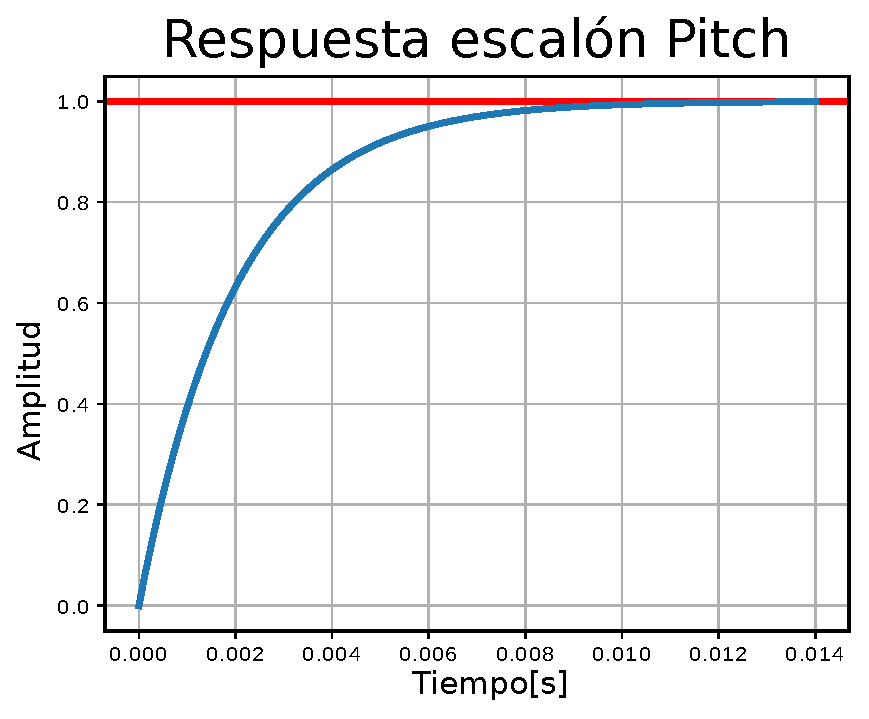
\includegraphics[width=0.7\textwidth]{Contenido/Cuerpo/Capitulo5/Fig35.eps}
	\captionof{figure}{Simulación entrada escalon}\label{Fig4}
\end{center}
Los valores para la ecuacion 5.14 se obtuvieron del trabajo de \cite{Paper::Abdo2013}, debido a la simulitud del sistema fisico, donde 
$J_{ay} = 0.002$ 

Como se abordo en el capitulo 3, el sistema dinamico de la gimbal es de primer orden para los movimientos en pitch y yaw, y como se definio en la seccion 5.1
el control que se implemento es el Proporcional-Integral. siendo este el necesario para hacer que el error converga a cero.\\
El diagrama de bloques de la figura 5.13 une todas las etapas de control, pasando por el control del servomotor, que hace una retroalimentación interna con base
en la dinamica vista en la seccion 5.1 y que obtenemos como salida el torque de entrada de la funcion de transferencia de la dinamica de Pitch para posteriormente
obtener la velocidad angular $q_a$, que despues pasa por un integrador y asi obtener la posición respecto al marco de referencia de la camara, es decir, en 
pixeles de la coordenada Y.
\begin{center}
	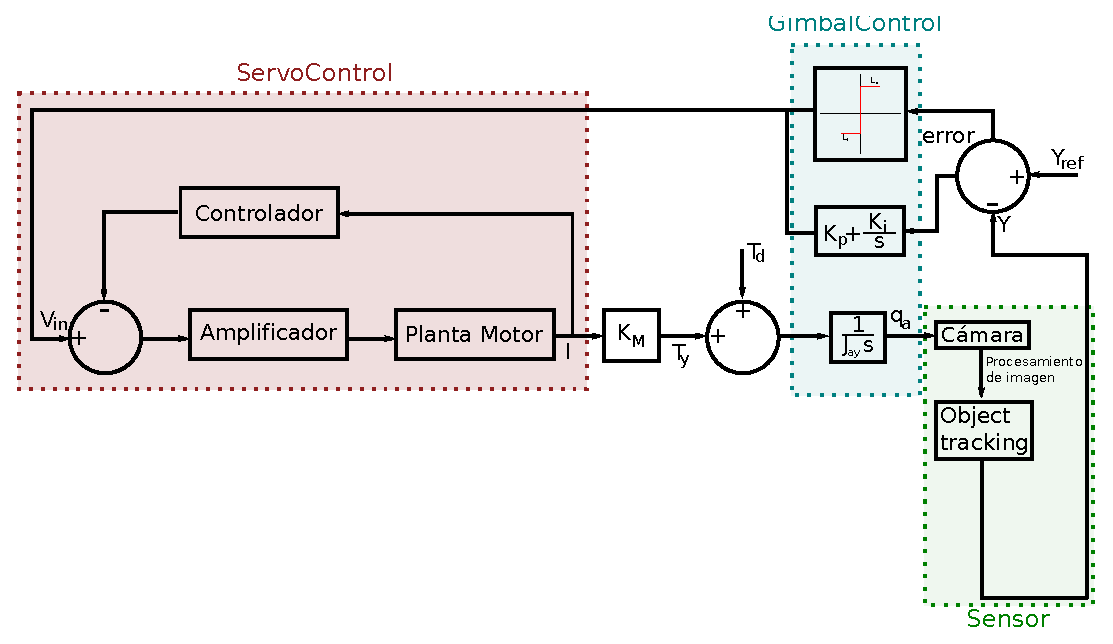
\includegraphics[width=1.0\textwidth]{Contenido/Cuerpo/Capitulo5/Fig22.eps}
	\captionof{figure}{Lazo de control para Pitch}\label{Fig4}
\end{center}
% Es un sistema de segundo orden retroalimentado por la camara y procesado en ROS. El lazo de control es aplicable también para la coordenada Y, como
% fue abordado en la sección 5.4 la comunicación se da mediante
% el protocolo serial, y debido a que la tarea que se encarga de realizar el algoritmo de control se debe suscribir al nodo de
% coordenadas, este se ve limitado, a un tiempo de muestreo de 60fps, o dicho de otro modo a 16.66 ms.

\subsubsection{Diseño de controlador}
El sistema tiene un controlador PI, donde tenemos la accion proporcional al error, que se encarga de acelerar la respuesta del sistema para llegar a la referencia
y tendra la accion integradora que se encarga de ajustar automaticamente el BIAS integrando el area bajo la curva del error presente en el proceso y de esa forma 
eliminar el error en estado estacionario. Tenemos que la función de transferencia del controlador PI viene dado por la expresion 
\begin{equation}
	C(s) = Kp(1 + \frac{1}{T_is})
\end{equation}
Donde $K_p$ es la ganancia proporcional y $T_i$ es el tiempo integral. La tecnica para el diseño del control se llama asignación de polos.\\
Aplicamos el lazo cerrado a la planta con el controlador, es decir $G_c(s) =  G(s)C(S)$
\begin{equation}
	G_c(s) = \frac{500K_ps + \frac{500K_p}{T_i}}{s^2 + 500K_ps + \frac{500K_p}{T_i}}
\end{equation}
De donde obtenemos la ecuacion caracteristica 
\begin{equation}
	E.C_1 = s^2 + 500K_ps + \frac{500K_p}{T_i}
\end{equation}
Como todavía no hemos definido cuales serán los parámetros del controlador PI, estos nos servirán para ubicar los polos en el lugar que nosotros queremos, es por 
eso que esta técnica es conocida como asignación de polos.\\
Como condiciones de diseño tenemos que considerar lo siguiente:
\begin{itemize}
	\item El sistema teoricamente podria establecerse en un tiempo de 0.01 segundos acorde a la figura 5.13, sin embardo fisicamente no es posible debido a dos 
		  factores, los motores ya tienen su lazo de control incluido como se detallo en la seccion 5.5.1 y la velocidad sin carga es de 0.14s lo cual es una
		  limitante y segundo el tiempo de muestreo de la camara es mayor al de establecimiento del control, ya que esta en 60Hz.
	\item Por lo anterior el tiempo de asentamiento $T_s$ se establece en 0.2s 
	\item El porcentaje de error se establece en 2\%
	\item Y el pico Maximo $M_p$ no debe pasar del 2\%
\end{itemize}
La función deseada que cumpla los puntos anteriores es de la forma 
\begin{equation}
	G_d(s) = \frac{\omega_n^2}{s^2 + 2\zeta\omega + \omega_n^2}
\end{equation}
donde el factor de amortiguamiento esta dado por
\begin{equation}
	\zeta = \sqrt{\frac{\ln\left(\frac{M_p}{100}\right)^2}{\pi^2 + \ln\left(\frac{M_p}{100}\right)^2}}
\end{equation}
y la frecuencia natural viene dada por la expresion
\begin{equation}
	\omega_n = \frac{3}{\zeta T_s}
\end{equation}
Apartir de las ecuaciones 5.19 y 5.20 y con los parametros de diseño obtenemos la funcionde transferencia con los polos deseados 
\begin{equation}
	Gd(s) = \frac{1086}{s^2 + 60s + 1086}
\end{equation}
La ecuacion caracteristica de la funcion de transferencia de la ecuacion 5.21 viene dada por la 
expresion 5.22
\begin{equation}
	E.C_2 = s^2 + 60s + 1086 = s^2 + \alpha_1s + \alpha_2
\end{equation}
Donde los polos deseados se situan en $s_{1,2} = -30, \pm 13.6437j$ \\
Igualamos la ecuacion 5.22 con 5.17 para calcular el valor de $K_p$ y $T_i$
\begin{equation}
	500K_p = \alpha_1
\end{equation}
\begin{equation}
	\frac{500K_p}{T_i} = \alpha_2
\end{equation}
Apartir de las ecuaciones 5.23 y 5.24 obtenemos los valores de $K_p = 0.118$ y $T_i = 0.054$, por lo que nuestro controlador viene dado por la siguiente 
ecuacion
\begin{equation}
	C(s) = 0.118 + \frac{2.1851}{s}
\end{equation}
El diagrama de la figura 5.15 muestra el lazo cerrado de controladorPI y la planta de PITCH
\begin{center}
	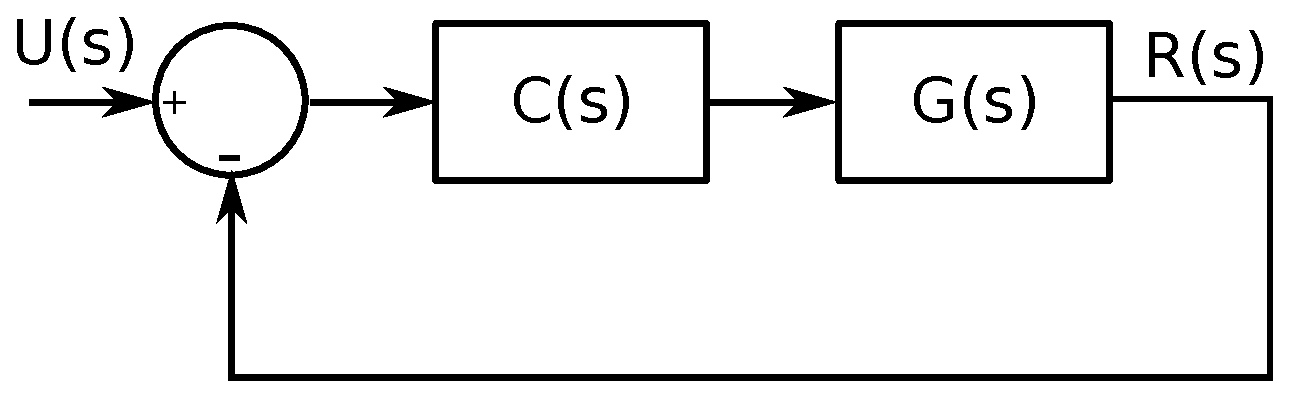
\includegraphics[width=0.6\textwidth]{Contenido/Cuerpo/Capitulo5/Fig37.eps}
	\captionof{figure}{Lazo cerrado del sistema con control PI}\label{Fig4}
\end{center}
Si aplicamos U(s) = 1, obtenemos la siguiente respuesta en el tiempo del sistema. 
\begin{center}
	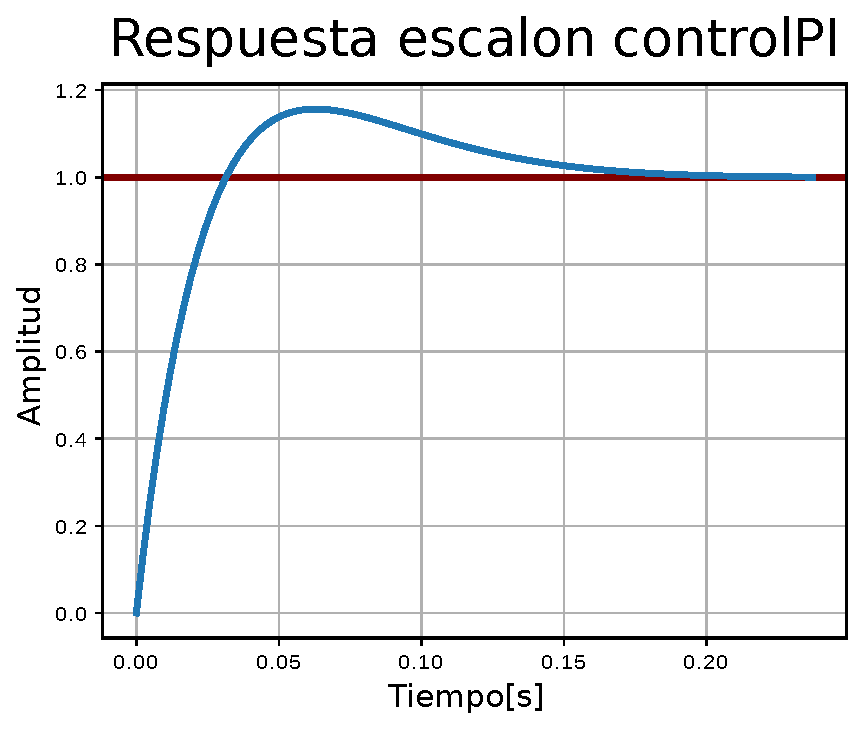
\includegraphics[width=0.6\textwidth]{Contenido/Cuerpo/Capitulo5/Fig38.eps}
	\captionof{figure}{Simulación respuesta escalon en PITCH}\label{Fig4}
\end{center}
La simulación de la figura 5.16 muestra que el sistema tiene un tiempo de establecimiento de 0.2 segundos tal y como se 
planeó en la etapa de diseño, hay un pequeño sobre impulso que en la practica no representara mas del 2\%. El codigo para 
la simulación esta hecho en python y puede ser consultado en mi repositorio de \href{https://github.com/MarcoAAG/Tesis}{\textbf{GitHub}}.
La Ganancia Ki de la ecuacion 5.25 se ve modificada en el microcontrolador debido a que se utiliza el metodo numerico para la integracion del error, por lo que 
la ganacia se multiplica por el tiempo de muestreo que es de 0.016, entonces la ecuacion 5.25 se convierte en:
\begin{equation}
	C(s) = 0.118 + \frac{0.034}{s}
\end{equation}
\subsubsection{Algortimo de control}
El algoritmo general del control tanto para pitch y para yaw esta descrito en el diagrama 5.17, basado en programación orientado a objetos
donde hay dos puntos claves, la obtención de datos de la camara via serial y la publicación de los errores para su posterior uso en graficas.
\begin{center}
	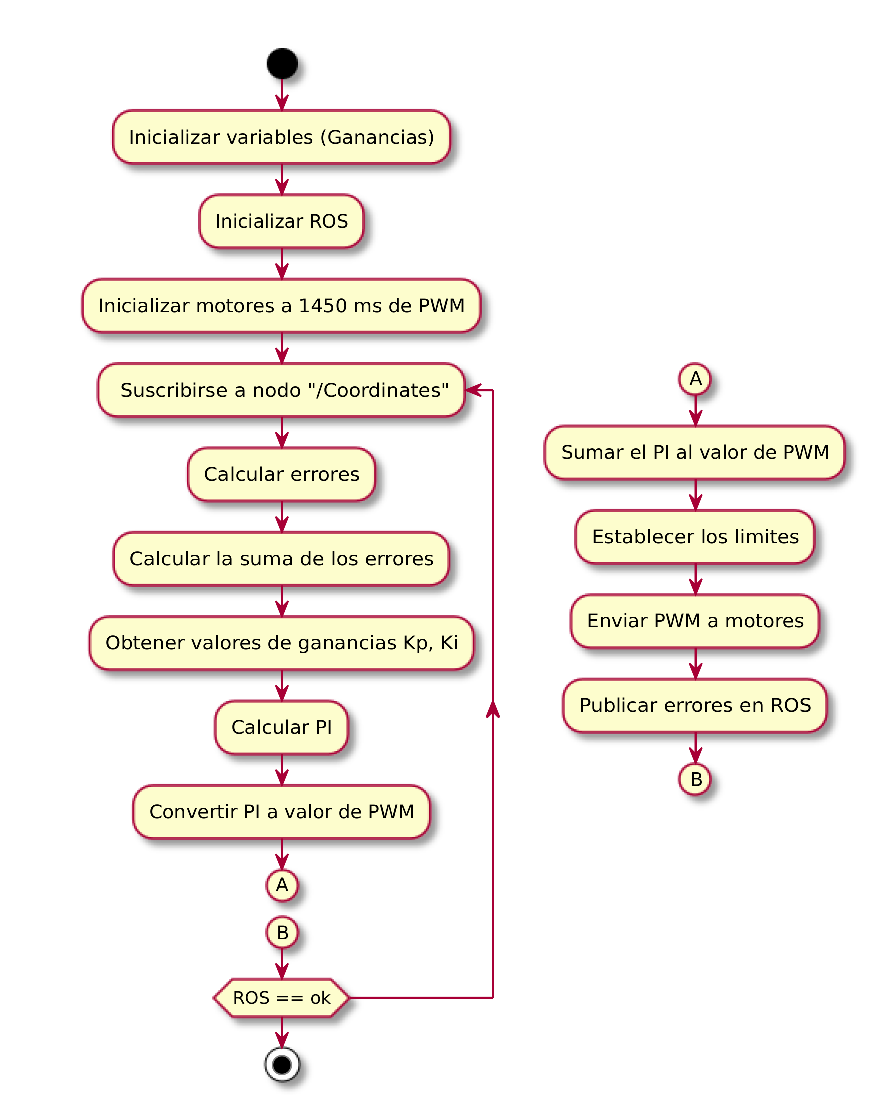
\includegraphics[width=0.6\textwidth]{Contenido/Cuerpo/Capitulo5/Fig24.eps}
	\captionof{figure}{Diagrama de flujo de algoritmo de control}\label{Fig4}
\end{center}
\subsubsection{Sintonización de control}
Lo primero que se realizo fue un controlador proporcional y se analizo su respuesta en el tiempo, de la cual se graficó el error, teniendo 
como referencia el cero.\\
La figura 5.18 muestra el resultado de sintonizar la ganancia Kp a uno, como se puede observar el sistema comienza en las primeras 50 muestras
para despues dar paso a un reposo, el error se mantiene en 20, por lo que el siguiente paso fue reducir la ganancia Kp
\begin{center}
	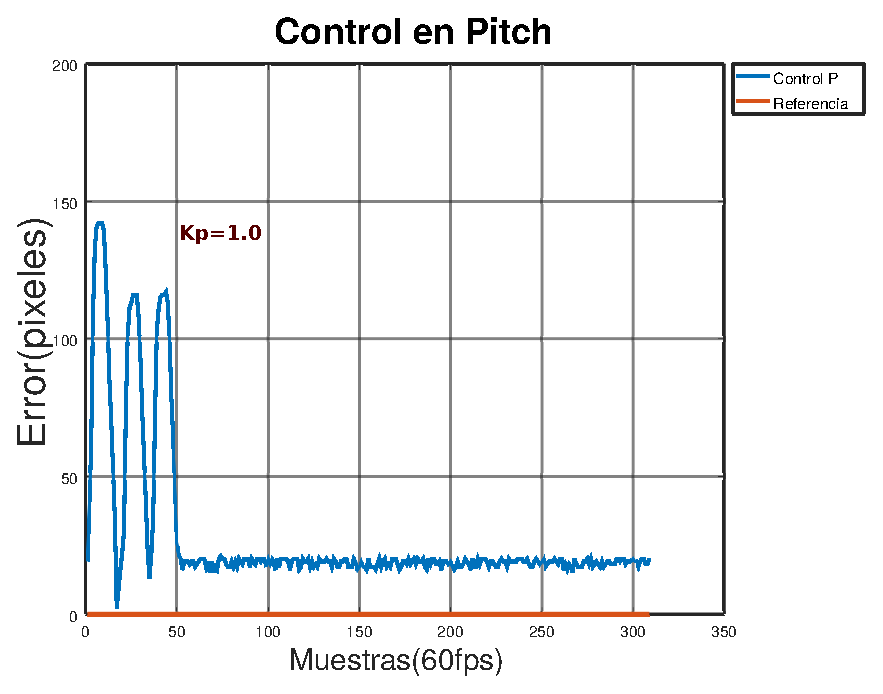
\includegraphics[width=0.83\textwidth]{Contenido/Cuerpo/Capitulo5/Fig25.eps}
	\captionof{figure}{Grafica del error en Pitch con ganancia Kp = 1}\label{Fig4}
\end{center}
Como abordó anteriormente las ganancias deseadas para el control PI se ubican por debajo de cero, por lo que la siguiente prueba fue bajar la ganancia Kp.
La figura 5.19 muestra la respuesta del sistema con un controlador proporcional con ganancia Kp = 0.5
\begin{center}
	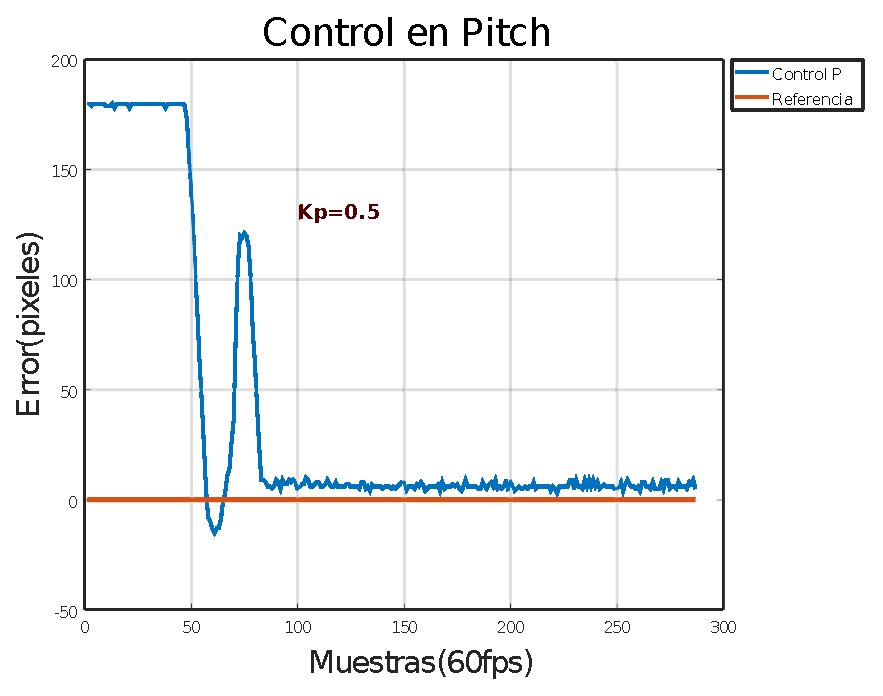
\includegraphics[width=0.8\textwidth]{Contenido/Cuerpo/Capitulo5/Fig26.eps}
	\captionof{figure}{Grafica del error en Pitch con ganancia Kp = 0.5}\label{Fig4}
\end{center}
Las oscilaciones antes de que se mantenga estable fueron menores en comparación con ganancia Kp, por lo que, el valor de la ganancia se 
redujo a 0.35, obteniendo como resultado la figura 5.20 
\begin{center}
	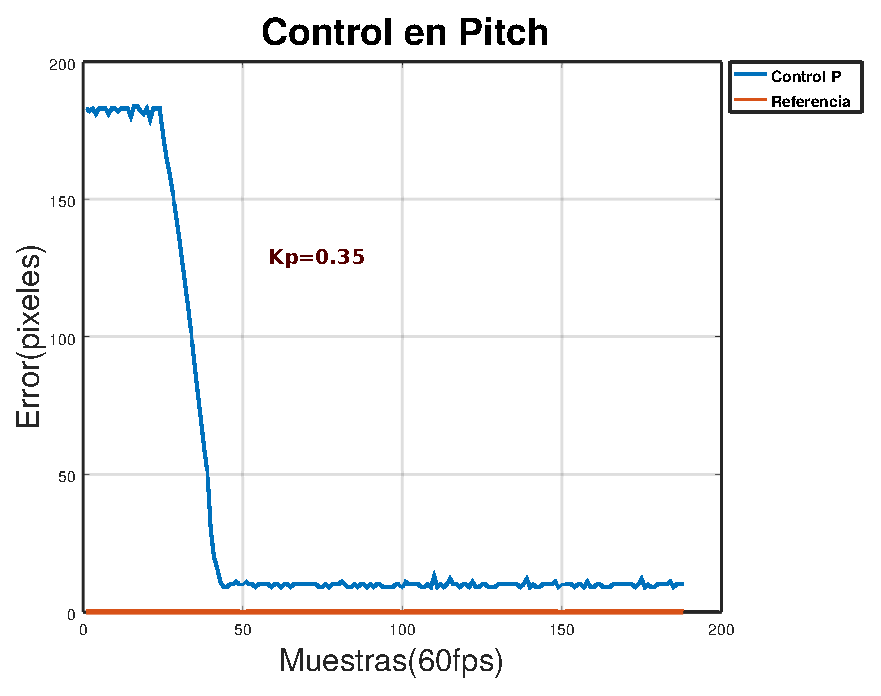
\includegraphics[width=0.8\textwidth]{Contenido/Cuerpo/Capitulo5/Fig27.eps}
	\captionof{figure}{Grafica del error en Pitch con ganancia Kp = 0.35}\label{Fig4}
\end{center}
Es claro que en la grafica 5.20 el sobre impulso es menor al 2\% sin embargo el error no converge a cero, se mantiene en 10, esto se 
puede solucionar con un control Integral, reducir el error en estado estacionario agregando la suma de los errores multiplicada por una ganacia 
Ki.Finalmante la grafica de la figura 5.21 muestra el resultado de agregar un controlador PI a la planta en Pitch, donde el error en estado 
estacionario es eliminado por la ganancia Ki, que a su vez ayuda a que el sistema converga en menor tiempo, donde se cumple una condición de diseño de $T_s = 0.2s$.
\begin{center}
	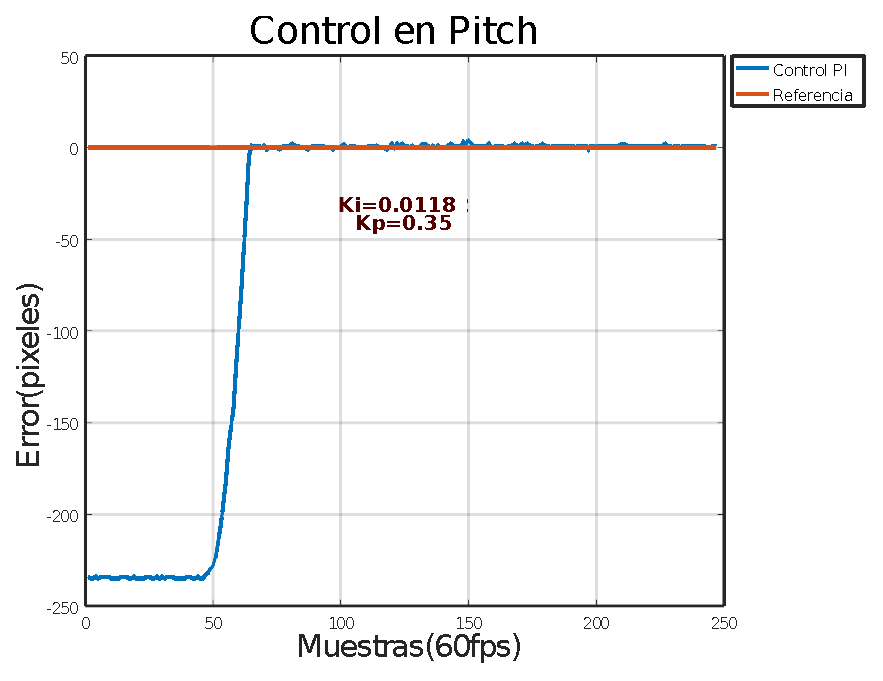
\includegraphics[width=0.8\textwidth]{Contenido/Cuerpo/Capitulo5/Fig28.eps}
	\captionof{figure}{Grafica del error en Pitch con control PI}\label{Fig4}
\end{center}

\subsection{Control en Yaw}
El sistema dinamico en Yaw es de primer orden, la obtencion de la ecuacion diferencial 
fue obtenida en el capitulo 3, de donde se obtuvo
\begin{equation}
	J_k\dot{r}_k = T_z+T_D
\end{equation}
Pasando la ecuacion 5.15 en el dominio de Laplace obtenemos
\begin{equation}
	J_{k}SR_k(s) = T_z(s)
\end{equation}
Dividimos entrada sobre salida, o en otras palabras, obtenemos la funcion de transferencia en lazo abierto
\begin{equation}
	G = \frac{R_k(s)}{T_z(s)} =  \frac{1}{J_{k}s}
\end{equation}
Y en lazo cerrado la ecuacion 5.29 se transforma en 
\begin{equation}
	G_c = \frac{G}{1 +GH} = \frac{1}{J_{k}s+1}
\end{equation}
Donde \\
$J_k = J_{kz} + J_{az} $ 
La figura 5.22 es el resultado de la simulación del sistema dinamico de pitch en lazo cerrado ante una entrada escalon.
\begin{center}
	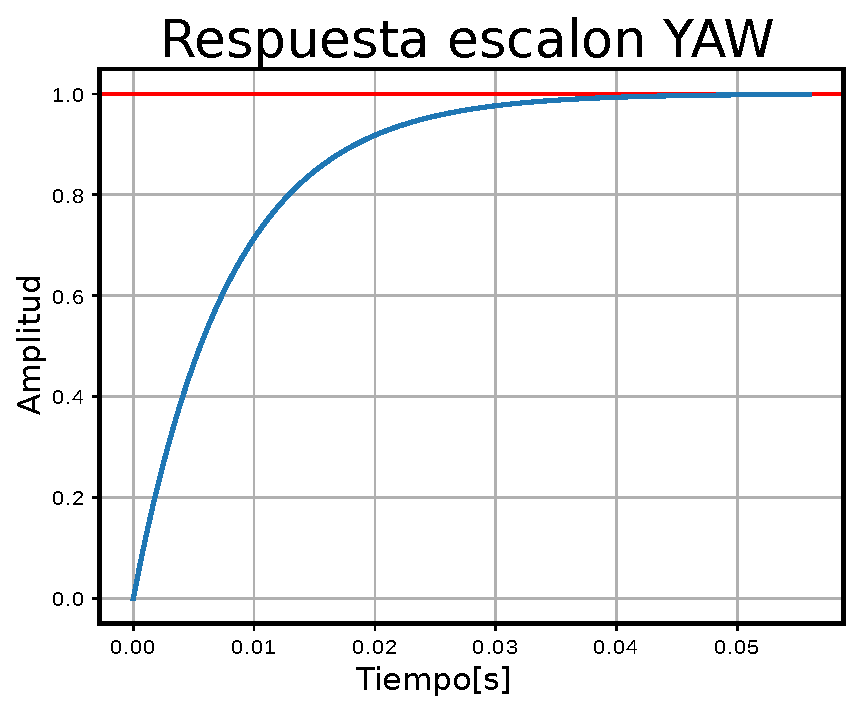
\includegraphics[width=0.6\textwidth]{Contenido/Cuerpo/Capitulo5/Fig39.eps}
	\captionof{figure}{Simulación entrada escalon para yaw}\label{Fig4}
\end{center}
Los valores para la ecuacion 5.30 se obtuvieron del trabajo de \cite{Paper::Abdo2013}, debido a la simulitud del sistema fisico, donde 
$J_{k} = 0.008$ 
De manera similar que en pitch tenemos un sistema de lazo cerrado donde se involucra el lazo de control del 
servomotor y la retroalimentación en la camara como se observa en la figura 5.23
\begin{center}
	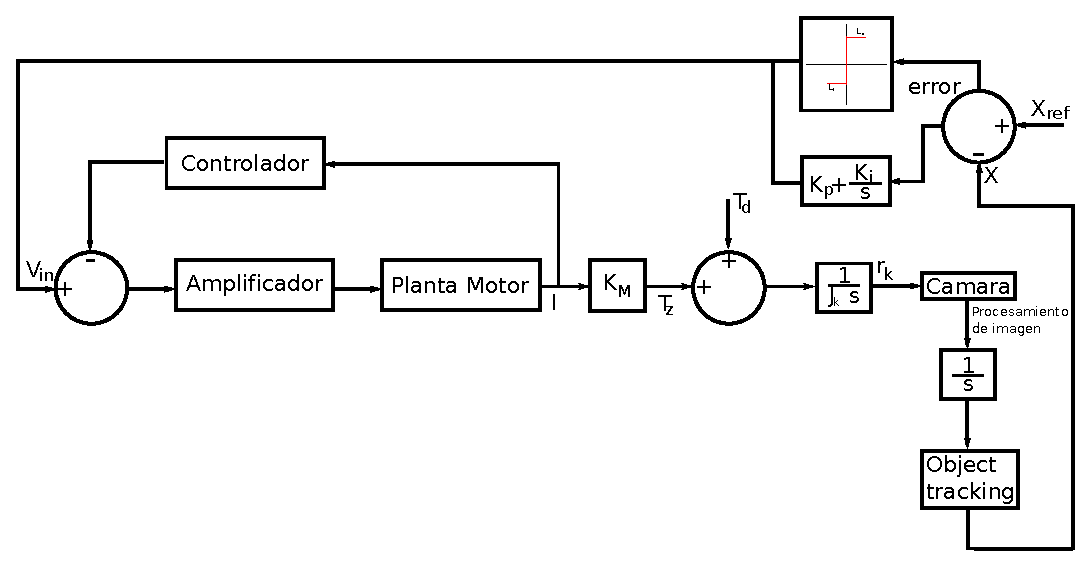
\includegraphics[width=0.95\textwidth]{Contenido/Cuerpo/Capitulo5/Fig34.eps}
	\captionof{figure}{Lazo de control para Yaw}\label{Fig4}
\end{center}
\subsubsection{Diseño de control}
De manera similar que en el control de Pitch en Yaw se diseñó un control PI debido a que dichos sitemas comparten comportamiento similares y se modelaron como sistemas de primer orden.
Para este sistema los parametros de diseño son los siguientes
\begin{itemize}
	\item $T_s$ = 0.3s
	\item Error menor al 2\%
	\item El Maximo sobre impulso no sobre pasa del 2\%
\end{itemize}
El procedimiento es el mismo que se abordo al diseñar el control para pitch, por lo que solo se agregan puntos claves del proceso.
La funcion de transferencia deseada se satisface las condiciones de diseño esta dada por la expresion 5.31
\begin{equation}
	G_d = \frac{482.7}{s^2 + 40s + 482.7}
\end{equation}
Donde los polos de la ecuación caracteristica se situan en $-20 \pm 9.0958j$\\
Despues de calcular la ganancia $K_p$ y el tiempo $T_i$ con base en los polos desados, obtenemos la funcion de trasferencia(ecuación 5.32) 
\begin{equation}
	G_c = 0.312 + \frac{3.8623}{s}
\end{equation}
Aplicando el lazo cerrado de la figura 5.15 y aplicando una entrada escalon se simuló la respuesta en el tiempo de la planta y el control.
\begin{center}
	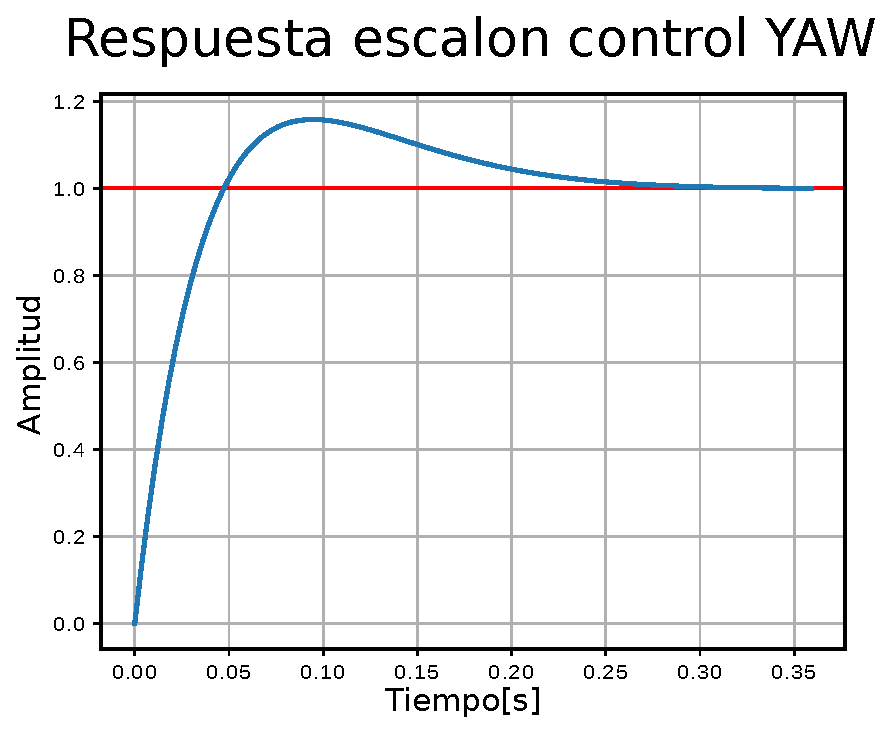
\includegraphics[width=0.65\textwidth]{Contenido/Cuerpo/Capitulo5/Fig40.eps}
	\captionof{figure}{Simulación del control PI en Yaw}\label{Fig4}
\end{center}
En la figura 5.24 podemos observar que el sistema simulado llega a la referencia en 0.3 segundos. Las ganancia que hacen que el sistema se comporte con los polos deseados son 
$K_p = 0.312$ y $K_i = 0.06179$\\
El controlador sigue el mismo algoritmo descrito en el diagrama 5.17
\subsubsection{Sintonización de control}
Para sintonizar el control PI primero se aplica ganancia Kp y se observa el comportmaiento del sistema, este
metodo nos ayuda a llegar lo mas cerca a la referencia, que en este caso es cero ya que estamos controlado
respecto a la dinamica del error. 
\begin{center}
	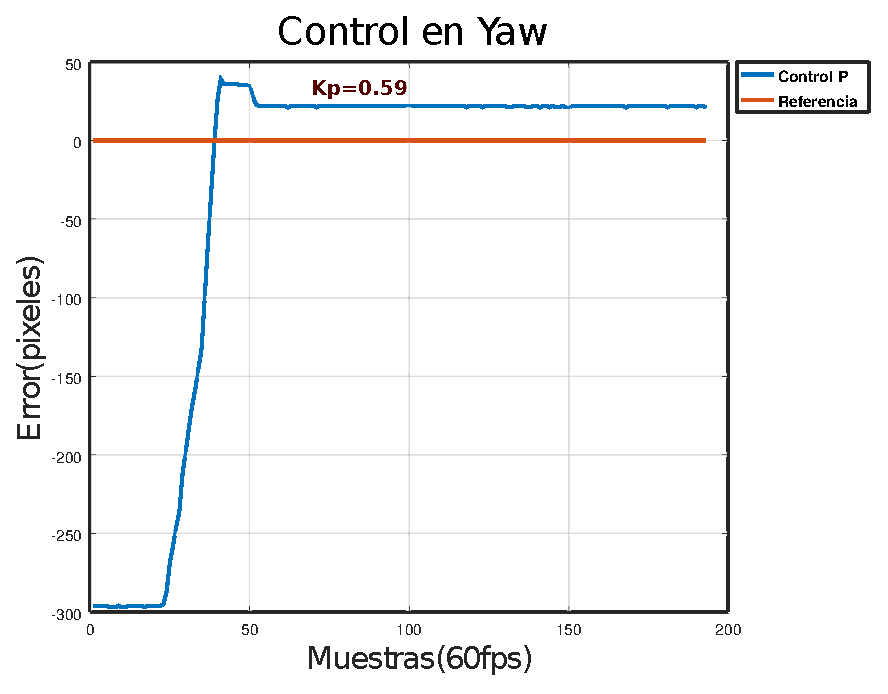
\includegraphics[width=0.83\textwidth]{Contenido/Cuerpo/Capitulo5/Fig30.eps}
	\captionof{figure}{Grafica del error en Yaw con ganancia Kp = 0.59}\label{Fig4}
\end{center}
La figura 5.25 muestra un control proporcional con ganancia mayor al 0.5, hay un sobre impulso que posteriormente 
hace que el sistema se mantenga con un error en 20 pixeles, le toma al sistema llegar a la referencia en 10 tiempos de 
muestreo, pero el control no se mantiene en error cero. Con base en la ganacia obtenida en la etapa de diseño del control la ganacia proporcional debe estar por debajo de 0.5.
\begin{center}
	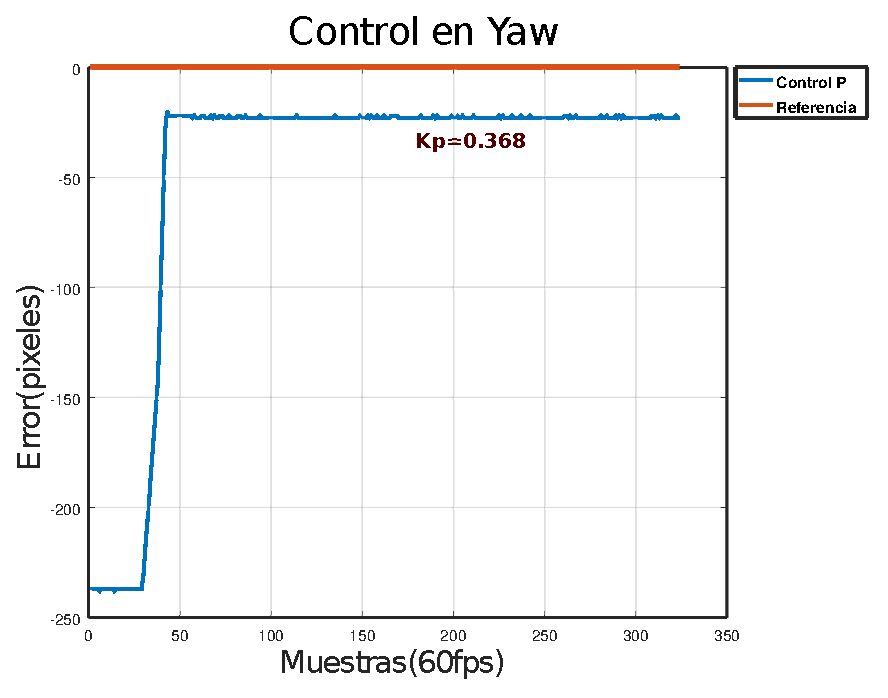
\includegraphics[width=0.83\textwidth]{Contenido/Cuerpo/Capitulo5/Fig31.eps}
	\captionof{figure}{Grafica del error en Yaw con ganancia Kp = 0.368}\label{Fig4}
\end{center}
Ahora la ganancia es menor que 0.5, lo que hace que el sistema no tenga un sobre impulso, pero tampoco llega 
a la referencia, se mantiene en un error de aproximadamente -20 pixeles, lo que tampoco es un comportamiento deseado.
La ganancia en 0.44 hace que el errror se mantenga cerano a cero (figura 5.24), con lo cual podemos aplicar la ganancia integral para erradicar el error ene stado estacionario 
\begin{center}
	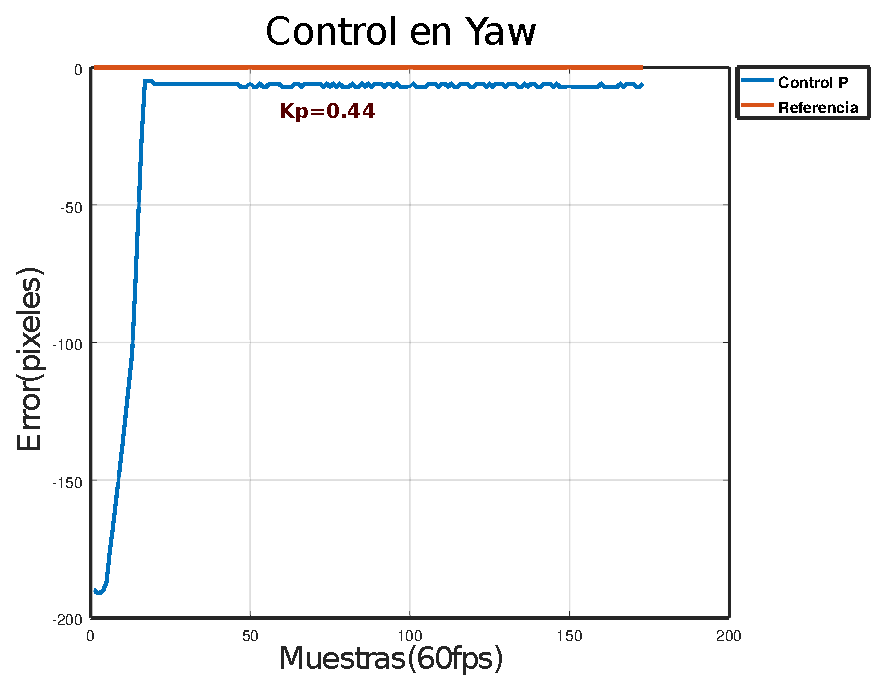
\includegraphics[width=0.83\textwidth]{Contenido/Cuerpo/Capitulo5/Fig32.eps}
	\captionof{figure}{Grafica del error en Yaw con ganancia Kp = 0.44}\label{Fig4}
\end{center}
Con una ganancia integral de 0.0351 el sistema se comporta como las especificaciones de diseño marcan, llegar a la referencia y mantenerse estable le toma al sistema 16 tiempos de 
muestreo, que equivalen a 0.3s y ademas el sobre impulso se ubica en menos del 2\% por lo que podemos decir que el control satisface los requerimientos.
\begin{center}
	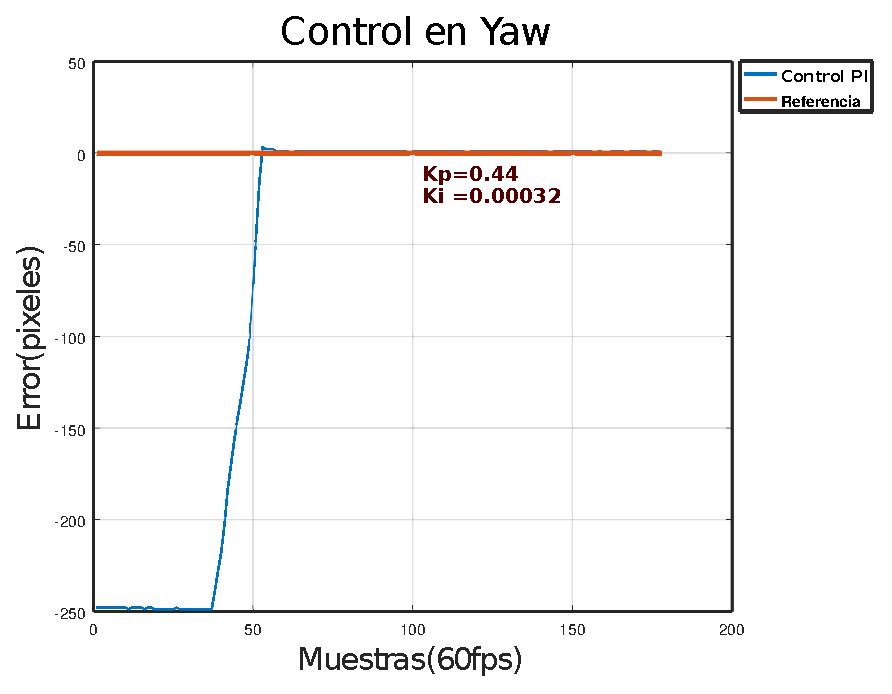
\includegraphics[width=0.83\textwidth]{Contenido/Cuerpo/Capitulo5/Fig33.eps}
	\captionof{figure}{Grafica del error en Yaw con control PI}\label{Fig4}
\end{center}